%  LaTeX support: latex@mdpi.com 
%  For support, please attach all files needed for compiling as well as the log file, and specify your operating system, LaTeX version, and LaTeX editor.

%=================================================================
\documentclass[journal,article,submit,pdftex,moreauthors]{Definitions/mdpi} 
%\documentclass[preprints,article,submit,pdftex,moreauthors]{Definitions/mdpi} 
% For posting an early version of this manuscript as a preprint, you may use "preprints" as the journal. Changing "submit" to "accept" before posting will remove line numbers.

% Below journals will use APA reference format:
% admsci, aieduc, behavsci, businesses, econometrics, economies, education, ejihpe, famsci, games, humans, ijcs, ijfs, jintelligence, journalmedia, jrfm, jsam, languages, peacestud, psycholint, publications, tourismhosp, youth

% Below journals will use Chicago reference format:
% arts, genealogy, histories, humanities, laws, literature, religions, risks, socsci

%--------------------
% Class Options:
%--------------------
%----------
% journal
%----------
% Choose between the following MDPI journals:
% accountaudit, acoustics, actuators, addictions, adhesives, admsci, adolescents, aerobiology, aerospace, agriculture, agriengineering, agrochemicals, agronomy, ai, aichem, aieduc, aieng, aimater, aimed, aipa, air, aisens, algorithms, allergies, alloys, amh, analog, analytica, analytics, anatomia, anesthres, animals, antibiotics, antibodies, antioxidants, applbiosci, appliedchem, appliedmath, appliedphys, applmech, applmicrobiol, applnano, applsci, aquacj, architecture, arm, arthropoda, arts, asc, asi, astronautics, astronomy, atmosphere, atoms, audiolres, automation, axioms, bacteria, batteries, bdcc, behavsci, beverages, biochem, bioengineering, biologics, biology, biomass, biomechanics, biomed, biomedicines, biomedinformatics, biomimetics, biomolecules, biophysica, bioresourbioprod, biosensors, biosphere, biotech, birds, blockchains, bloods, blsf, brainsci, breath, buildings, businesses, cancers, carbon, cardio, cardiogenetics, cardiovascmed, catalysts, cells, ceramics, challenges, chemengineering, chemistry, chemosensors, chemproc, children, chips, cimb, civileng, cleantechnol, climate, clinbioenerg, clinpract, clockssleep, cmd, cmtr, coasts, coatings, colloids, colorants, commodities, complexities, complications, compounds, computation, computers, condensedmatter, conservation, constrmater, cosmetics, covid, crops, cryo, cryptography, crystals, csmf, ctn, culture, curroncol, cyber, dairy, data, ddc, dentistry, dermato, dermatopathology, designs, devices, dhi, diabetology, diagnostics, dietetics, digital, disabilities, diseases, diversity, dna, drones, dynamics, earth, ebj, ecm, ecologies, econometrics, economies, edm, education, eesp, ejihpe, electricity, electrochem, electronicmat, electronics, encyclopedia, endocrines, energies, eng, engproc, entomology, entropy, environments, environremediat, epidemiologia, epigenomes, esa, est, famsci, fermentation, fibers, fintech, fire, fishes, fluids, foods, forecasting, forensicsci, forests, fossstud, foundations, fractalfract, fuels, future, futureinternet, futurepharmacol, futurephys, futuretransp, galaxies, games, gases, gastroent, gastrointestdisord, gastronomy, gels, genealogy, genes, geographies, geohazards, geomatics, geometry, geosciences, geotechnics, geriatrics, germs, glacies, grasses, green, greenhealth, gucdd, hardware, hazardousmatters, healthcare, hearts, hemato, hematolrep, hep, heritage, higheredu, highthroughput, histories, horticulturae, hospitals, humanities, humans, hydrobiology, hydrogen, hydrology, hydropower, hygiene, idr, iic, ijcs, ijem, ijerph, ijfs, ijgi, ijmd, ijms, ijns, ijom, ijpb, ijt, ijtm, ijtpp, ime, immuno, informatics, information, infrastructures, inorganics, insects, instruments, inventions, iot, j, jaestheticmed, jal, jcdd, jcm, jcp, jcrm, jcs, jcto, jdad, jdb, jdream, jemr, jeta, jfb, jfmk, jgbg, jgg, jimaging, jintelligence, jlpea, jmahp, jmmp, jmms, jmp, jmse, jne, jnt, jof, joi, joitmc, joma, jop, joptm, jor, journalmedia, jox, jpbi, jphytomed, jpm, jrfm, jsam, jsan, jtaer, jvd, jzbg, kidneydial, kinasesphosphatases, knowledge, labmed, laboratories, lae, land, languages, laws, life, lights, limnolrev, lipidology, liquids, literature, livers, logics, logistics, lubricants, lymphatics, machines, macromol, magnetism, magnetochemistry, make, marinedrugs, materials, materproc, mathematics, mca, measurements, medicina, medicines, medsci, membranes, merits, metabolites, metals, meteorology, methane, metrics, metrology, micro, microarrays, microbiolres, microelectronics, micromachines, microorganisms, microplastics, microwave, minerals, mining, mmphys, modelling, molbank, molecules, mps, msf, mti, multimedia, muscles, nanoenergyadv, nanomanufacturing, nanomaterials, ncrna, ndt, network, neuroglia, neuroimaging, neurolint, neurosci, nitrogen, notspecified, nursrep, nutraceuticals, nutrients, obesities, occuphealth, oceans, ohbm, onco, optics, oral, organics, organoids, osteology, oxygen, pandemics, parasites, parasitologia, particles, pathogens, pathophysiology, peacestud, pediatrrep, pets, pharmaceuticals, pharmaceutics, pharmacoepidemiology, pharmacy, philosophies, photochem, photonics, phycology, physchem, physics, physiologia, plants, plasma, platforms, pollutants, polymers, polysaccharides, populations, poultry, powders, precipitation, precisoncol, preprints, proceedings, processes, prosthesis, proteomes, psf, psychiatryint, psychoactives, psycholint, publications, purification, quantumrep, quaternary, qubs, radiation, rdt, reactions, realestate, receptors, recycling, regeneration, religions, remotesensing, reports, reprodmed, resources, rheumato, risks, rjpm, robotics, rsee, ruminants, safety, sci, scipharm, sclerosis, seeds, sensors, separations, sexes, shi, signals, sinusitis, siuj, skins, smartcities, sna, societies, socsci, software, soilsystems, solar, solids, spectroscj, sports, standards, stats, std, stratsediment, stresses, surfaces, surgeries, suschem, sustainability, symmetry, synbio, systems, tae, targets, taxonomy, technologies, telecom, test, textiles, thalassrep, therapeutics, thermo, timespace, tomography, tourismhosp, toxics, toxins, tph, transplantology, transportation, traumacare, traumas, tri, tropicalmed, universe, urbansci, uro, vaccines, vehicles, venereology, vetsci, vibration, virtualworlds, viruses, vision, waste, water, welding, wem, wevj, wild, wind, women, world, youth, zoonoticdis

%---------
% article
%---------
% The default type of manuscript is "article", but can be replaced by: 
% abstract, addendum, article, benchmark, book, bookreview, briefcommunication, briefreport, casereport, changes, clinicopathologicalchallenge, comment, commentary, communication, conceptpaper, conferenceproceedings, correction, conferencereport, creative, datadescriptor, discussion, entry, expressionofconcern, extendedabstract, editorial, essay, erratum, fieldguide, hypothesis, interestingimages, letter, meetingreport, monograph, newbookreceived, obituary, opinion, proceedingpaper, projectreport, reply, retraction, review, perspective, protocol, shortnote, studyprotocol, supfile, systematicreview, technicalnote, viewpoint, guidelines, registeredreport, tutorial,  giantsinurology, urologyaroundtheworld
% supfile = supplementary materials

%----------
% submit
%----------
% The class option "submit" will be changed to "accept" by the Editorial Office when the paper is accepted. This will only make changes to the frontpage (e.g., the logo of the journal will get visible), the headings, and the copyright information. Also, line numbering will be removed. Journal info and pagination for accepted papers will also be assigned by the Editorial Office.

%------------------
% moreauthors
%------------------
% If there is only one author the class option oneauthor should be used. Otherwise use the class option moreauthors.

%---------
% pdftex
%---------
% The option pdftex is for use with pdfLaTeX. Remove "pdftex" for (1) compiling with LaTeX & dvi2pdf (if eps figures are used) or for (2) compiling with XeLaTeX.

%=================================================================
% MDPI internal commands - do not modify
\firstpage{1} 
\makeatletter 
\setcounter{page}{\@firstpage} 
\makeatother
\pubvolume{1}
\issuenum{1}
\articlenumber{0}
\pubyear{2026}
\copyrightyear{2026}
%\externaleditor{Firstname Lastname} % More than 1 editor, please add `` and '' before the last editor name
\datereceived{ } 
\daterevised{ } % Comment out if no revised date
\dateaccepted{ } 
\datepublished{ } 
%\datecorrected{} % For corrected papers: "Corrected: XXX" date in the original paper.
%\dateretracted{} % For retracted papers: "Retracted: XXX" date in the original paper.
%\doinum{} % Used for some special journals, like molbank
%\pdfoutput=1 % Uncommented for upload to arXiv.org
%\CorrStatement{yes}  % For updates
%\longauthorlist{yes} % For many authors that exceed the left citation part
%\IsAssociation{yes} % For association journals

%=================================================================
% Add packages and commands here. The following packages are loaded in our class file: fontenc, inputenc, calc, indentfirst, fancyhdr, graphicx, epstopdf, lastpage, ifthen, float, amsmath, amssymb, lineno, setspace, enumitem, mathpazo, booktabs, titlesec, etoolbox, tabto, xcolor, colortbl, soul, multirow, microtype, tikz, totcount, changepage, attrib, upgreek, array, tabularx, pbox, ragged2e, tocloft, marginnote, marginfix, enotez, amsthm, natbib, hyperref, cleveref, scrextend, url, geometry, newfloat, caption, draftwatermark, seqsplit
% cleveref: load \crefname definitions after \begin{document}

%=================================================================
% Please use the following mathematics environments: Theorem, Lemma, Corollary, Proposition, Characterization, Property, Problem, Example, ExamplesandDefinitions, Hypothesis, Remark, Definition, Notation, Assumption
%% For proofs, please use the proof environment (the amsthm package is loaded by the MDPI class).

%=================================================================
% Full title of the paper (Capitalized)
\Title{Prompting vs. Parameter-Efficient Fine-Tuning for JSON Extraction from Noisy User Commands}

% Author Orchid ID: enter ID or remove command
\newcommand{\orcidauthorA}{0009-0004-4210-5756}%RK
\newcommand{\orcidauthorB}{0000-0002-3015-1024}%Sandi
\newcommand{\orcidauthorC}{0000-0003-0323-2600}%Vedran
\newcommand{\orcidauthorD}{0000-0002-5964-245X}%Ivan

% Authors, for the paper (add full first names)
\Author{Ratomir Karlović $^{1}$\orcidA{}, Sandi Baressi Šegota $^{1,}$*\orcidB{}, Vedran Mrzljak $^{2,}$*\orcidC{} and Ivan Lorencin $^{1}$\orcidD{}}

%\longauthorlist{yes}

% MDPI internal command: Authors, for metadata in PDF
\AuthorNames{Ratomir Karlović, Sandi Baressi Šegota, Vedran Mrzljak and Ivan Lorencin}

%\longauthorlist{yes}

% Affiliations / Addresses (Add [1] after \address if there is only one affiliation.)
\address{%
$^{1}$ \quad Faculty of Informatics, Juraj Dobrila University of Pula, Zagrebačka 30, 52100 Pula, Croatia;\\ ratomir.karlovic@unipu.hr (R.K.), sandi.baressi.segota@unipu.hr (S.B.Š.), ivan.lorencin@unipu.hr (I.L.)\\ $^{2}$ \quad Faculty of Engineering Rijeka, University of Rijeka, Vukovarska 58, 51000 Rijeka, Croatia; vedran.mrzljak@riteh.uniri.hr (V.M.)}

% Contact information of the corresponding author
\corres{Correspondence: sandi.baressi.segota@unipu.hr; vedran.mrzljak@riteh.uniri.hr}

% Current address and/or shared authorship
%\firstnote{Current address: Affiliation.}  
% Current address should not be the same as any items in the Affiliation section.

%\secondnote{These authors contributed equally to this work.}
% The commands \thirdnote{} till \eighthnote{} are available for further notes.

%\simplesumm{} % Simple summary

%\conference{} % An extended version of a conference paper

% Abstract (Do not insert blank lines, i.e. \\) 
\abstract{A single paragraph of about 200 words maximum. For research articles, abstracts should give a pertinent overview of the work. We strongly encourage authors to use the following style of structured abstracts, but without headings: (1) Background: place the question addressed in a broad context and highlight the purpose of the study; (2) Methods: describe briefly the main methods or treatments applied; (3) Results: summarize the article's main findings; (4) Conclusions: indicate the main conclusions or interpretations. The abstract should be an objective representation of the article, it must not contain results which are not presented and substantiated in the main text and should not exaggerate the main conclusions.}

% Keywords
\keyword{keyword 1; keyword 2; keyword 3 (List three to ten pertinent keywords specific to the article; yet reasonably common within the subject discipline.)} 

% The fields PACS, MSC, and JEL may be left empty or commented out if not applicable
%\PACS{J0101}
%\MSC{}
%\JEL{}

%%%%%%%%%%%%%%%%%%%%%%%%%%%%%%%%%%%%%%%%%%
% Only for the journal Diversity
%\LSID{\url{http://}}

%%%%%%%%%%%%%%%%%%%%%%%%%%%%%%%%%%%%%%%%%%
% Only for the journal Applied Sciences
%\featuredapplication{Authors are encouraged to provide a concise description of the specific application or a potential application of the work. This section is not mandatory.}
%%%%%%%%%%%%%%%%%%%%%%%%%%%%%%%%%%%%%%%%%%

%%%%%%%%%%%%%%%%%%%%%%%%%%%%%%%%%%%%%%%%%%
% Only for the journal Data
%\dataset{DOI number or link to the deposited data set if the data set is published separately. If the data set shall be published as a supplement to this paper, this field will be filled by the journal editors. In this case, please submit the data set as a supplement.}
%\datasetlicense{License under which the data set is made available (CC0, CC-BY, CC-BY-SA, CC-BY-NC, etc.)}

%%%%%%%%%%%%%%%%%%%%%%%%%%%%%%%%%%%%%%%%%%
% Only for the journal BioTech, Fishes, Neuroimaging and Toxins
%\keycontribution{The breakthroughs or highlights of the manuscript. Authors can write one or two sentences to describe the most important part of the paper.}

%%%%%%%%%%%%%%%%%%%%%%%%%%%%%%%%%%%%%%%%%%
% Only for the journal Encyclopedia
%\encyclopediadef{For entry manuscripts only: please provide a brief overview of the entry title instead of an abstract.}

%%%%%%%%%%%%%%%%%%%%%%%%%%%%%%%%%%%%%%%%%%
% Different journals have different requirements. Please check the specific journal guidelines in the "Instructions for Authors" on the journal's official website.
%\addhighlights{yes}
%\renewcommand{\addhighlights}{%
%
%\noindent The goal is to increase the discoverability and readability of the article via search engines and other scholars. Highlights should not be a copy of the abstract, but a simple text allowing the reader to quickly and simplified find out what the article is about and what can be cited from it. Each of these parts should be devoted up to 2~bullet points.\vspace{3pt}\\
%\textbf{What are the main findings?}
% \begin{itemize}[labelsep=2.5mm,topsep=-3pt]
% \item First bullet.
% \item Second bullet.
% \end{itemize}\vspace{3pt}
%\textbf{What are the implications of the main findings?}
% \begin{itemize}[labelsep=2.5mm,topsep=-3pt]
% \item First bullet.
% \item Second bullet.
% \end{itemize}
%}

%%%%%%%%%%%%%%%%%%%%%%%%%%%%%%%%%%%%%%%%%%
\begin{document}

%%%%%%%%%%%%%%%%%%%%%%%%%%%%%%%%%%%%%%%%%%

\section{Introduction}

The template details the sections that can be used in a manuscript. Note that the order and names of article sections may differ from the requirements of the journal (e.g., the positioning of the Materials and Methods section). Please check the instructions on the authors' page of the journal to verify the correct order and names. For any questions, please contact the editorial office of the journal or support@mdpi.com. For LaTeX-related questions please contact latex@mdpi.com.%\endnote{This is an endnote.} % To use endnotes, please un-comment \printendnotes below (before References). Only journal Laws uses \footnote.

% The order of the section titles is different for some journals. Please refer to the "Instructions for Authors” on the journal homepage.

\section{Background and Related Work}

% The introduction should briefly place the study in a broad context and highlight why it is important. It should define the purpose of the work and its significance. The current state of the research field should be reviewed carefully and key publications cited. Please highlight controversial and diverging hypotheses when necessary. Finally, briefly mention the main aim of the work and highlight the principal conclusions. As far as possible, please keep the introduction comprehensible to scientists outside your particular field of research. Citing a journal paper \citep{ref-journal}.  Now citing a book reference \citep{ref-book1,ref-book2} or other reference types \citep{ref-unpublish,ref-url}. Please use the command \citep{ref-proceeding,ref-thesis} for the following MDPI journals, which use author--date citation: Administrative Sciences, Arts, Behavioral Sciences, Businesses, Econometrics, Economies, Education Sciences, European Journal of Investigation in Health, Psychology and Education, Games, Genealogy, Histories, Humanities, Humans, IJFS, Journal of Intelligence, Journalism and Media, JRFM, Languages, Laws, Literature, Psychology International, Publications, Religions, Risks, Social Sciences, Tourism and Hospitality, Youth. 

%%%%%%%%%%%%%%%%%%%%%%%%%%%%%%%%%%%%%%%%%%
\section{Methodology}\label{sec:methods}

This section describes how we built the data, ran the models and evaluated their outputs. We first define the task and the four noise tiers, and then describe the training, validation and test data. Next, we describe the two models, the two inference setups and the three prompts used without fine-tuning, followed by the two adapter methods and their training settings. The section ends with the evaluation metrics, the efficiency measurements and the statistical tests.

\subsection{Task and Output Format}\label{sec:task}

Each input is a single natural-language command that changes a shopping cart. The model must return one JSON object with three fields: \texttt{action}, \texttt{product} and \texttt{quantity}. The action is one of \texttt{add}, \texttt{remove} or \texttt{update}. The product is a free-text string that names one item, and the quantity is an integer between 1 and 30. A command such as ``Throw out 18 lychees from the cart.'' maps to \texttt{\{"action": "remove", "product": "lychees", "quantity": 18\}}. Every command contains exactly one action, one product and one quantity.

\subsection{Noise Tiers}\label{sec:tiers}

Each command exists in four parallel versions, called tiers. All four versions of a command share the same correct output. Tier~0 is a clean, direct command. Tier~1 adds lexical noise to the Tier~0 sentence: it is lowercased, punctuation is removed, some words lose vowels, and some commands end with a slang token (\texttt{asap}, \texttt{rn}, \texttt{thx} or \texttt{pls}). Tier~2 expresses the same request in conversational form, with fillers, hesitations and politeness phrases. Tier~3 contains a spontaneous self-correction: the user first states a wrong quantity and then corrects it, so the last stated quantity is the correct one. In Tier~3, only the quantity is corrected; the action and the product stay the same. Table~\ref{tab:tiers} shows one command from the test set in all four tiers.

\begin{table}[H]
\caption{Noise tiers. One test-set command in all four tiers; the correct output for every tier is \texttt{\{"action": "add", "product": "beef brisket", "quantity": 14\}}.\label{tab:tiers}}
\begin{tabularx}{\textwidth}{lp{3.2cm}X}
\toprule
Tier & Noise type & Example \\
\midrule
0 & None (clean) & Grab fourteen beef brisket. \\
1 & Lexical & grb fourteen bf brskt pls \\
2 & Conversational & So, uh, yeah, put fourteen beef brisket, I think. \\
3 & Self-correction & Pop in 21 beef brisket, no sorry, fourteen. \\
\bottomrule
\end{tabularx}
\end{table}

\subsection{Datasets}\label{sec:data}

We used three datasets with the same format: a training set, a validation set and a test set. Each row of a dataset holds one command in all four tiers together with its three output labels. The training and validation sets were used to train the adapters and to select their checkpoints, and the test set was used for all reported results. The training and validation data come from one generation process, while the test set was built separately with new products and new sentence templates, as described below.

\subsubsection{Training and Validation Data}\label{sec:data-train}

The training and validation sets were generated by prompting Claude Opus 5.5, as two separate files: 9600 commands for training and 1200 for validation. The model was instructed to produce rows in a fixed CSV format, each row containing the three output labels and the four tier versions of one command. The instructions specified the three allowed actions, quantities between 1 and 30 written as digits or as words (for example, ``a dozen'' or ``twenty''), a product vocabulary of retail items from several categories (groceries, produce, household goods, electronics, office supplies and apparel), and the noise definitions of Section~\ref{sec:tiers}. Because every command has four tiers, the two sets contain 38,400 training and 4800 validation examples.

Table~\ref{tab:data} summarizes the datasets. The training and validation commands use 250 distinct products, and all validation products also occur in the training set. The generated sentences follow a small number of patterns. When the product name and all quantity expressions are replaced by placeholders, the 9600 training commands contain only 62 distinct Tier~0 templates and 48 distinct Tier~3 templates. In Tier~1 of the training set, 18.8\% of words longer than three characters were changed, 29.5\% of commands end with a slang token, and the product name is unchanged in 75.8\% of commands.

\subsubsection{Test Set}\label{sec:data-test}

Because the training data are highly templated, a test set drawn from the same generation process would mainly test whether a model recognizes training templates. We therefore built a separate test set with new products and new sentence templates. The test set was generated with Claude Opus 5.5 using a seeded, template-based procedure. It contains 1200 commands (4800 inputs over the four tiers), with 400 commands per action and every quantity from 1 to 30 (28 to 53 commands per value). Quantities are written as digits in 50.2\% of Tier~0 commands and as words in the rest.

The test set differs from the training data in three ways. First, it uses 176 products, none of which occurs in the training or validation data. Second, no masked sentence template of Tiers~0, 2 or~3 occurs in the training or validation data, and no command string is repeated. Third, it uses more varied sentence patterns: 269 Tier~0, 1151 Tier~2 and 475 Tier~3 templates. Tier~1 noise follows the same procedure as in the training data: each word longer than three characters is changed with a probability of 0.18 by deleting one or more of its vowels, and a slang token is appended to 30\% of commands. The measured rates match the training data: 18.2\% of non-product words and 19.2\% of product words were changed, 28.7\% of commands end with a slang token, and the product name is unchanged in 72.9\% of commands. Because the test sentences are longer, a larger share of Tier~1 commands contains at least one changed word (54.1\% compared with 42.0\% in the training set).

To keep the labels unambiguous, every test command names its action with a verb or phrase that belongs to only one action. For example, ``throw out'' and ``subtract'' are used only for \texttt{remove}, and ``revise'' and ``set'' only for \texttt{update}. Verbs that can signal more than one action, such as ``drop'' (``drop in'' versus ``drop''), were not used. Update commands always contain an explicit update verb. Quantity forms that need a following noun, such as ``a pair of'', appear only directly before the product. We checked every test command with a separate rule-based checker that uses its own action lexicon and number parser. For each of the 3600 commands in Tiers~0, 2 and~3, the checker confirmed that the text names the labeled action, contains the labeled product exactly once, and states the labeled quantity; in Tier~3, it confirmed that all earlier quantities equal the wrong value and that the last one equals the label. For Tier~1, it confirmed that every change from Tier~0 is a vowel deletion. All commands passed these checks.

\begin{table}[H]
\caption{Dataset summary. Inputs count every command once per tier. Products not in the training set are products that do not occur in any training command. Templates are counted after replacing the product name and all quantity expressions with placeholders. Tier~1 templates are not counted because each Tier~1 command is its Tier~0 sentence with random vowel deletions, so its template is the Tier~0 template.\label{tab:data}}
\begin{tabularx}{\textwidth}{lCCC}
\toprule
 & Training & Validation & Test \\
\midrule
Commands & 9600 & 1200 & 1200 \\
Inputs (four tiers) & 38,400 & 4800 & 4800 \\
\midrule
Commands with action add & 3233 & 402 & 400 \\
Commands with action remove & 3288 & 400 & 400 \\
Commands with action update & 3079 & 398 & 400 \\
\midrule
Distinct products & 250 & 249 & 176 \\
Products not in the training set & 0 & 0 & 176 \\
\midrule
Tier~0 templates & 62 & 50 & 269 \\
Tier~2 templates & 315 & 231 & 1151 \\
Tier~3 templates & 48 & 42 & 475 \\
\bottomrule
\end{tabularx}
\end{table}

\subsection{Models and Inference Setups}\label{sec:models}

We used two instruction-tuned open-weight models: Llama~3.2~3B~Instruct and Llama~3.1~8B~Instruct~\citep{grattafiori2024llama}, referred to below as the 3B and 8B models. Each model was run without fine-tuning in two inference setups, which differ in quantization format, prompt formatting and output decoding.

In the Ollama setup, we used the \texttt{llama3.2:3b} and \texttt{llama3.1:8b} models in the Q4\_K\_M 4-bit format. Generation used a temperature of 0 and no limit on the output length. The target JSON schema was passed through the \texttt{format} parameter, which restricts the output to a JSON object with the three required fields and their types (two strings and one integer). The schema does not restrict the action to the three allowed values or the quantity to the range 1--30.

In the Transformers setup, we used the Hugging Face Transformers library and loaded the models in 4-bit NF4 quantization with double quantization and bfloat16 compute~\citep{dettmers2023qlora}. Generation used greedy decoding with at most 64 new tokens and no output constraint. The input was formatted with each model's chat template, with a limit of 512 input tokens; the longest input had 236 tokens, so no input was truncated. The adapters described in Section~\ref{sec:peft} were trained and evaluated on the same 4-bit base models with the same generation settings. Differences between the Transformers baseline and an adapter therefore come from the adapter alone. Comparisons between the Ollama and Transformers setups compare two complete inference setups, because several factors differ between them.

In both setups, the prompt was passed as the system message and the command as the user message. Of all 115,200 generated outputs, 556 (0.5\%) reached the limit of 64 new tokens. All of them were schema-invalid for other reasons: 548 consisted of explanatory text instead of a JSON object, and 8 began a JSON object but repeated the same characters until the limit, so the limit did not change any reported result. All experiments ran on a single NVIDIA A100 GPU with 40~GB of memory on a high-performance computing cluster. Software versions are listed in the code repository.

\subsection{Prompt Designs}\label{sec:prompts}

We tested three prompts; their full texts are given in Appendix~\ref{app:prompts}. The minimal prompt contains one sentence that names the task and a JSON template with the three fields. The extended prompt adds a role description, an instruction to use the final value when the user corrects an earlier statement, the list of allowed actions, and an instruction not to add markdown or explanations. The few-shot prompt is the extended prompt plus three input--output examples: one add command, one remove command and one add command with a quantity correction. None of the three example products occurs in the test set.

\subsection{Parameter-Efficient Fine-Tuning}\label{sec:peft}

We trained two types of adapters, LoRA and IA$^3$, which leave the base model weights unchanged and train a small number of added parameters.

LoRA~\citep{hu2022lora} keeps each adapted weight matrix frozen and adds a trainable update to it. The update is the product of two small matrices with rank $r$, scaled by $\alpha / r$, so only these two matrices are trained. We applied LoRA to the query, key, value and output projections of every attention layer (\texttt{q\_proj}, \texttt{k\_proj}, \texttt{v\_proj}, \texttt{o\_proj}).

IA$^3$~\citep{liu2022fewshot} adds no new matrices. Instead, it learns one vector for each adapted activation and multiplies the activation element-wise by this vector. In our setup, IA$^3$ rescales the keys and values in every attention layer and the input of the feed-forward down projection (\texttt{down\_proj}). Because it trains only these vectors, IA$^3$ has far fewer trainable parameters than LoRA (Table~\ref{tab:peft}).

We trained one adapter for each combination of model (3B, 8B), adapter type (LoRA, IA$^3$) and prompt (minimal, extended, few-shot), which gives 12 adapters. Each adapter was trained with the same prompt that was used to evaluate it. A training example consists of the prompt, the command and the target JSON object, formatted with the model's chat template. All four tiers of every training command were used, and the loss was computed over the full formatted sequence. Table~\ref{tab:peft} lists the training settings. The checkpoint with the lowest validation loss was kept as the final adapter.

\begin{table}[H]
\caption{Adapter training settings. The base model was loaded in 4-bit NF4 quantization and kept frozen in all runs.\label{tab:peft}}
\begin{tabularx}{\textwidth}{lCC}
\toprule
Setting & LoRA & IA$^3$ \\
\midrule
Target modules & \texttt{q\_proj}, \texttt{k\_proj}, \texttt{v\_proj}, \texttt{o\_proj} & \texttt{k\_proj}, \texttt{v\_proj}, \texttt{down\_proj} \\
Rank $r$ & 16 & -- \\
Scaling $\alpha$ & 32 & -- \\
Dropout & 0.05 & -- \\
Trainable parameters, 3B model & 9,175,040 & 286,720 \\
Trainable parameters, 8B model & 13,631,488 & 524,288 \\
Learning rate & $2 \times 10^{-4}$ & $1 \times 10^{-3}$ \\
\midrule
\multicolumn{3}{l}{Shared settings} \\
Epochs & \multicolumn{2}{c}{3 (7200 optimizer steps)} \\
Batch size & \multicolumn{2}{c}{1 per step, 16 gradient-accumulation steps (effective 16)} \\
Warm-up & \multicolumn{2}{c}{3\% of steps, then linear decay} \\
Optimizer & \multicolumn{2}{c}{Paged 8-bit AdamW} \\
Precision & \multicolumn{2}{c}{bfloat16, gradient checkpointing} \\
Maximum sequence length & \multicolumn{2}{c}{512 tokens} \\
Checkpoint selection & \multicolumn{2}{c}{Lowest validation loss, evaluated after each epoch} \\
Random seed & \multicolumn{2}{c}{42} \\
\bottomrule
\end{tabularx}
\end{table}

\subsection{Evaluation Metrics}\label{sec:metrics}

Each model output was parsed as follows. A surrounding markdown code block was removed if present, and the remaining text had to be a single JSON object with exactly the keys \texttt{action}, \texttt{product} and \texttt{quantity}. The action and product had to be non-empty strings, and the quantity had to be an integer. Outputs that failed any of these checks were counted as schema-invalid. For a test set of $N$ inputs, schema adherence is
\begin{equation}
\mathrm{SA} = \frac{100}{N} \sum_{i=1}^{N} v_i,
\label{eq:sa}
\end{equation}
where $v_i = 1$ if output $i$ is schema-valid and $v_i = 0$ otherwise. Schema adherence does not check whether the field values are correct.

Before comparison, the action and product strings were lowercased and runs of whitespace were reduced to a single space. No other normalization was applied: a misspelled or pluralized product name counts as wrong. The exact match rate (EMR) is the percentage of inputs for which all three fields equal the reference:
\begin{equation}
\mathrm{EMR} = \frac{100}{N} \sum_{i=1}^{N} v_i \, \mathbb{1}\!\left[\hat{a}_i = a_i \wedge \hat{p}_i = p_i \wedge \hat{q}_i = q_i\right],
\label{eq:emr}
\end{equation}
where $a_i$, $p_i$ and $q_i$ are the reference action, product and quantity, $\hat{a}_i$, $\hat{p}_i$ and $\hat{q}_i$ are the predicted values, and $\mathbb{1}[\cdot]$ is 1 if the condition holds and 0 otherwise. A schema-invalid output never counts as a match. To locate errors, we also report field accuracy, the percentage of inputs for which a single field is correct; schema-invalid outputs count as wrong for every field. EMR is the main metric. All metrics were computed separately for each tier.

\subsection{Efficiency Measurement}\label{sec:efficiency}

We measured generation speed, energy use and GPU memory. Generation speed is the number of output tokens divided by generation time. In the Ollama setup, generation time is the duration reported by Ollama for producing the output tokens. In the Transformers setup and for the adapters, it is the measured time of each generation call, which also includes processing the input. Speed values are therefore comparable within a setup but not between the Ollama and Transformers setups.

Energy use was measured with the CodeCarbon library. A separate measurement covered each run of 1200 inputs (one model, setup, prompt and tier), and we report the total energy in kilowatt-hours. In preliminary runs, the first measurement in each job reported a GPU power of 0~W. We therefore started and discarded a 20~s measurement before the first recorded measurement of each job; all reported runs show non-zero GPU power. For the adapters, we also recorded the peak GPU memory allocated during training and during inference.

\subsection{Statistical Analysis}\label{sec:stats}

For each EMR value, we report a 95\% Wilson confidence interval~\citep{wilson1927probable}. With $k$ exact matches out of $n$ inputs, $\hat{\pi} = k/n$ and $z = 1.96$, the interval is
\begin{equation}
\frac{\hat{\pi} + \frac{z^2}{2n} \pm z \sqrt{\frac{\hat{\pi}(1-\hat{\pi})}{n} + \frac{z^2}{4n^2}}}{1 + \frac{z^2}{n}}.
\label{eq:wilson}
\end{equation}

Because all methods were evaluated on the same inputs, we compared methods with the exact McNemar test~\citep{mcnemar1947note}. For two methods A and B on the same tier, let $b$ be the number of inputs that only A answered correctly and $c$ the number that only B answered correctly. Under the null hypothesis of equal accuracy, $b$ follows a binomial distribution with $b + c$ trials and probability 0.5, and we report the two-sided $p$-value of this test. Before the analysis, we fixed four comparisons: LoRA versus the Transformers baseline, IA$^3$ versus the Transformers baseline, LoRA versus IA$^3$, and the Ollama setup versus the Transformers setup. Each comparison was made for both models, all three prompts and all four tiers, which gives 96 tests. We corrected the $p$-values for multiple testing with the Holm method~\citep{holm1979simple} over all 96 tests and report a difference as significant if the corrected $p$-value is below 0.05.

We ran the complete evaluation twice. All reported numbers come from the second run, in which energy was measured as described in Section~\ref{sec:efficiency}; the first run serves as a reproducibility check (Section~\ref{sec:results}).

%%%%%%%%%%%%%%%%%%%%%%%%%%%%%%%%%%%%%%%%%%
\section{Results and Discussion}\label{sec:results}

This section first reports the results and then discusses them. We start with the overall exact match rate of every method and then look at how it changes with the noise tier and the prompt. Next, we examine which output fields fail and why, and test which differences between methods are statistically significant. The results end with the training and inference cost of each method and a check of how reproducible the runs were. Section~\ref{sec:discussion} then answers the research questions. All numbers come from the second of the two complete evaluation runs (Section~\ref{sec:stats}).

\subsection{Overall Accuracy}\label{sec:res-overall}

Table~\ref{tab:emr} lists the exact match rate (EMR) for every model, prompt, method and tier. Over all four tiers, LoRA reached between 92.2\% and 95.1\% for both models and all three prompts. Without adapters, the few-shot prompt gave the best results: 83.5\% in the Ollama setup and 81.7\% in the Transformers setup for the 3B model, and 85.5\% and 84.8\% for the 8B model. IA$^3$ reached between 63.1\% and 76.7\% with the 3B model and between 79.5\% and 89.4\% with the 8B model. The half-width of the 95\% Wilson confidence interval was between 0.5 and 2.8 percentage points for every tier value in the table.

Schema adherence was high in most configurations. With the extended and few-shot prompts, at least 97.0\% of the outputs were schema-valid on every tier, both with and without adapters. LoRA produced schema-valid outputs for at least 99.5\% of the inputs with every prompt. The exceptions were the Transformers baseline with the minimal prompt and, to a smaller degree, IA$^3$ with the minimal prompt; Section~\ref{sec:res-prompts} describes them.

\begin{table}[H]
\caption{Exact match rate (EMR, \%) on the test set for each model, prompt, method and tier. Each tier has 1200 inputs; the last column covers all 4800 inputs. The half-width of the 95\% Wilson confidence interval is between 0.5 and 2.8 percentage points for every tier value.\label{tab:emr}}
\begin{tabularx}{\textwidth}{lllCCCCC}
\toprule
Model & Prompt & Method & Tier~0 & Tier~1 & Tier~2 & Tier~3 & All tiers \\
\midrule
3B & Minimal & Ollama & 11.0 & 9.5 & 10.4 & 6.0 & 9.2 \\
 &  & Transformers & 2.2 & 1.2 & 0.6 & 0.8 & 1.2 \\
 &  & IA$^3$ & 80.4 & 56.6 & 60.0 & 55.3 & 63.1 \\
 &  & LoRA & 95.6 & 83.6 & 97.2 & 97.2 & 93.4 \\
\midrule
 & Extended & Ollama & 89.8 & 60.4 & 85.4 & 59.0 & 73.7 \\
 &  & Transformers & 87.8 & 59.4 & 85.6 & 63.3 & 74.0 \\
 &  & IA$^3$ & 87.4 & 60.8 & 81.3 & 77.2 & 76.7 \\
 &  & LoRA & 95.4 & 83.1 & 95.6 & 94.7 & 92.2 \\
\midrule
 & Few-shot & Ollama & 92.7 & 67.2 & 91.1 & 82.9 & 83.5 \\
 &  & Transformers & 91.9 & 64.8 & 88.4 & 81.7 & 81.7 \\
 &  & IA$^3$ & 83.8 & 62.4 & 79.2 & 77.1 & 75.6 \\
 &  & LoRA & 98.2 & 82.7 & 96.3 & 97.3 & 93.6 \\
\midrule
8B & Minimal & Ollama & 16.2 & 12.0 & 11.9 & 5.2 & 11.3 \\
 &  & Transformers & 7.3 & 5.0 & 6.2 & 1.2 & 4.9 \\
 &  & IA$^3$ & 89.8 & 64.8 & 82.7 & 80.8 & 79.5 \\
 &  & LoRA & 95.9 & 85.0 & 95.9 & 93.6 & 92.6 \\
\midrule
 & Extended & Ollama & 96.4 & 67.5 & 94.1 & 59.8 & 79.4 \\
 &  & Transformers & 95.8 & 64.9 & 90.5 & 70.3 & 80.4 \\
 &  & IA$^3$ & 97.9 & 70.3 & 97.4 & 86.8 & 88.1 \\
 &  & LoRA & 97.1 & 85.8 & 96.3 & 96.3 & 93.9 \\
\midrule
 & Few-shot & Ollama & 95.2 & 66.2 & 93.5 & 87.1 & 85.5 \\
 &  & Transformers & 95.0 & 64.4 & 92.2 & 87.6 & 84.8 \\
 &  & IA$^3$ & 98.2 & 70.8 & 98.1 & 90.3 & 89.4 \\
 &  & LoRA & 98.0 & 86.8 & 97.6 & 98.0 & 95.1 \\
\bottomrule
\end{tabularx}
\end{table}

\subsection{Effect of Noise Tiers}\label{sec:res-tiers}

The tiers differed strongly in difficulty, and the order did not follow the tier numbers. Figures~\ref{fig:emr_tiers_3b} and~\ref{fig:emr_tiers_8b} show the EMR per tier with the few-shot prompt. Tier~1 (lexical noise) had the lowest EMR in 17 of the 24 configurations, including all six LoRA configurations. The seven exceptions were the four baselines with the minimal prompt, whose EMR stayed below 17\% on every tier, the Ollama setup with the extended prompt, and IA$^3$ with the 3B model and the minimal prompt. In these seven configurations, Tier~3 had the lowest EMR, except for the 3B Transformers baseline with the minimal prompt, where all four tiers stayed between 0.6\% and 2.2\%.

\begin{figure}[H]
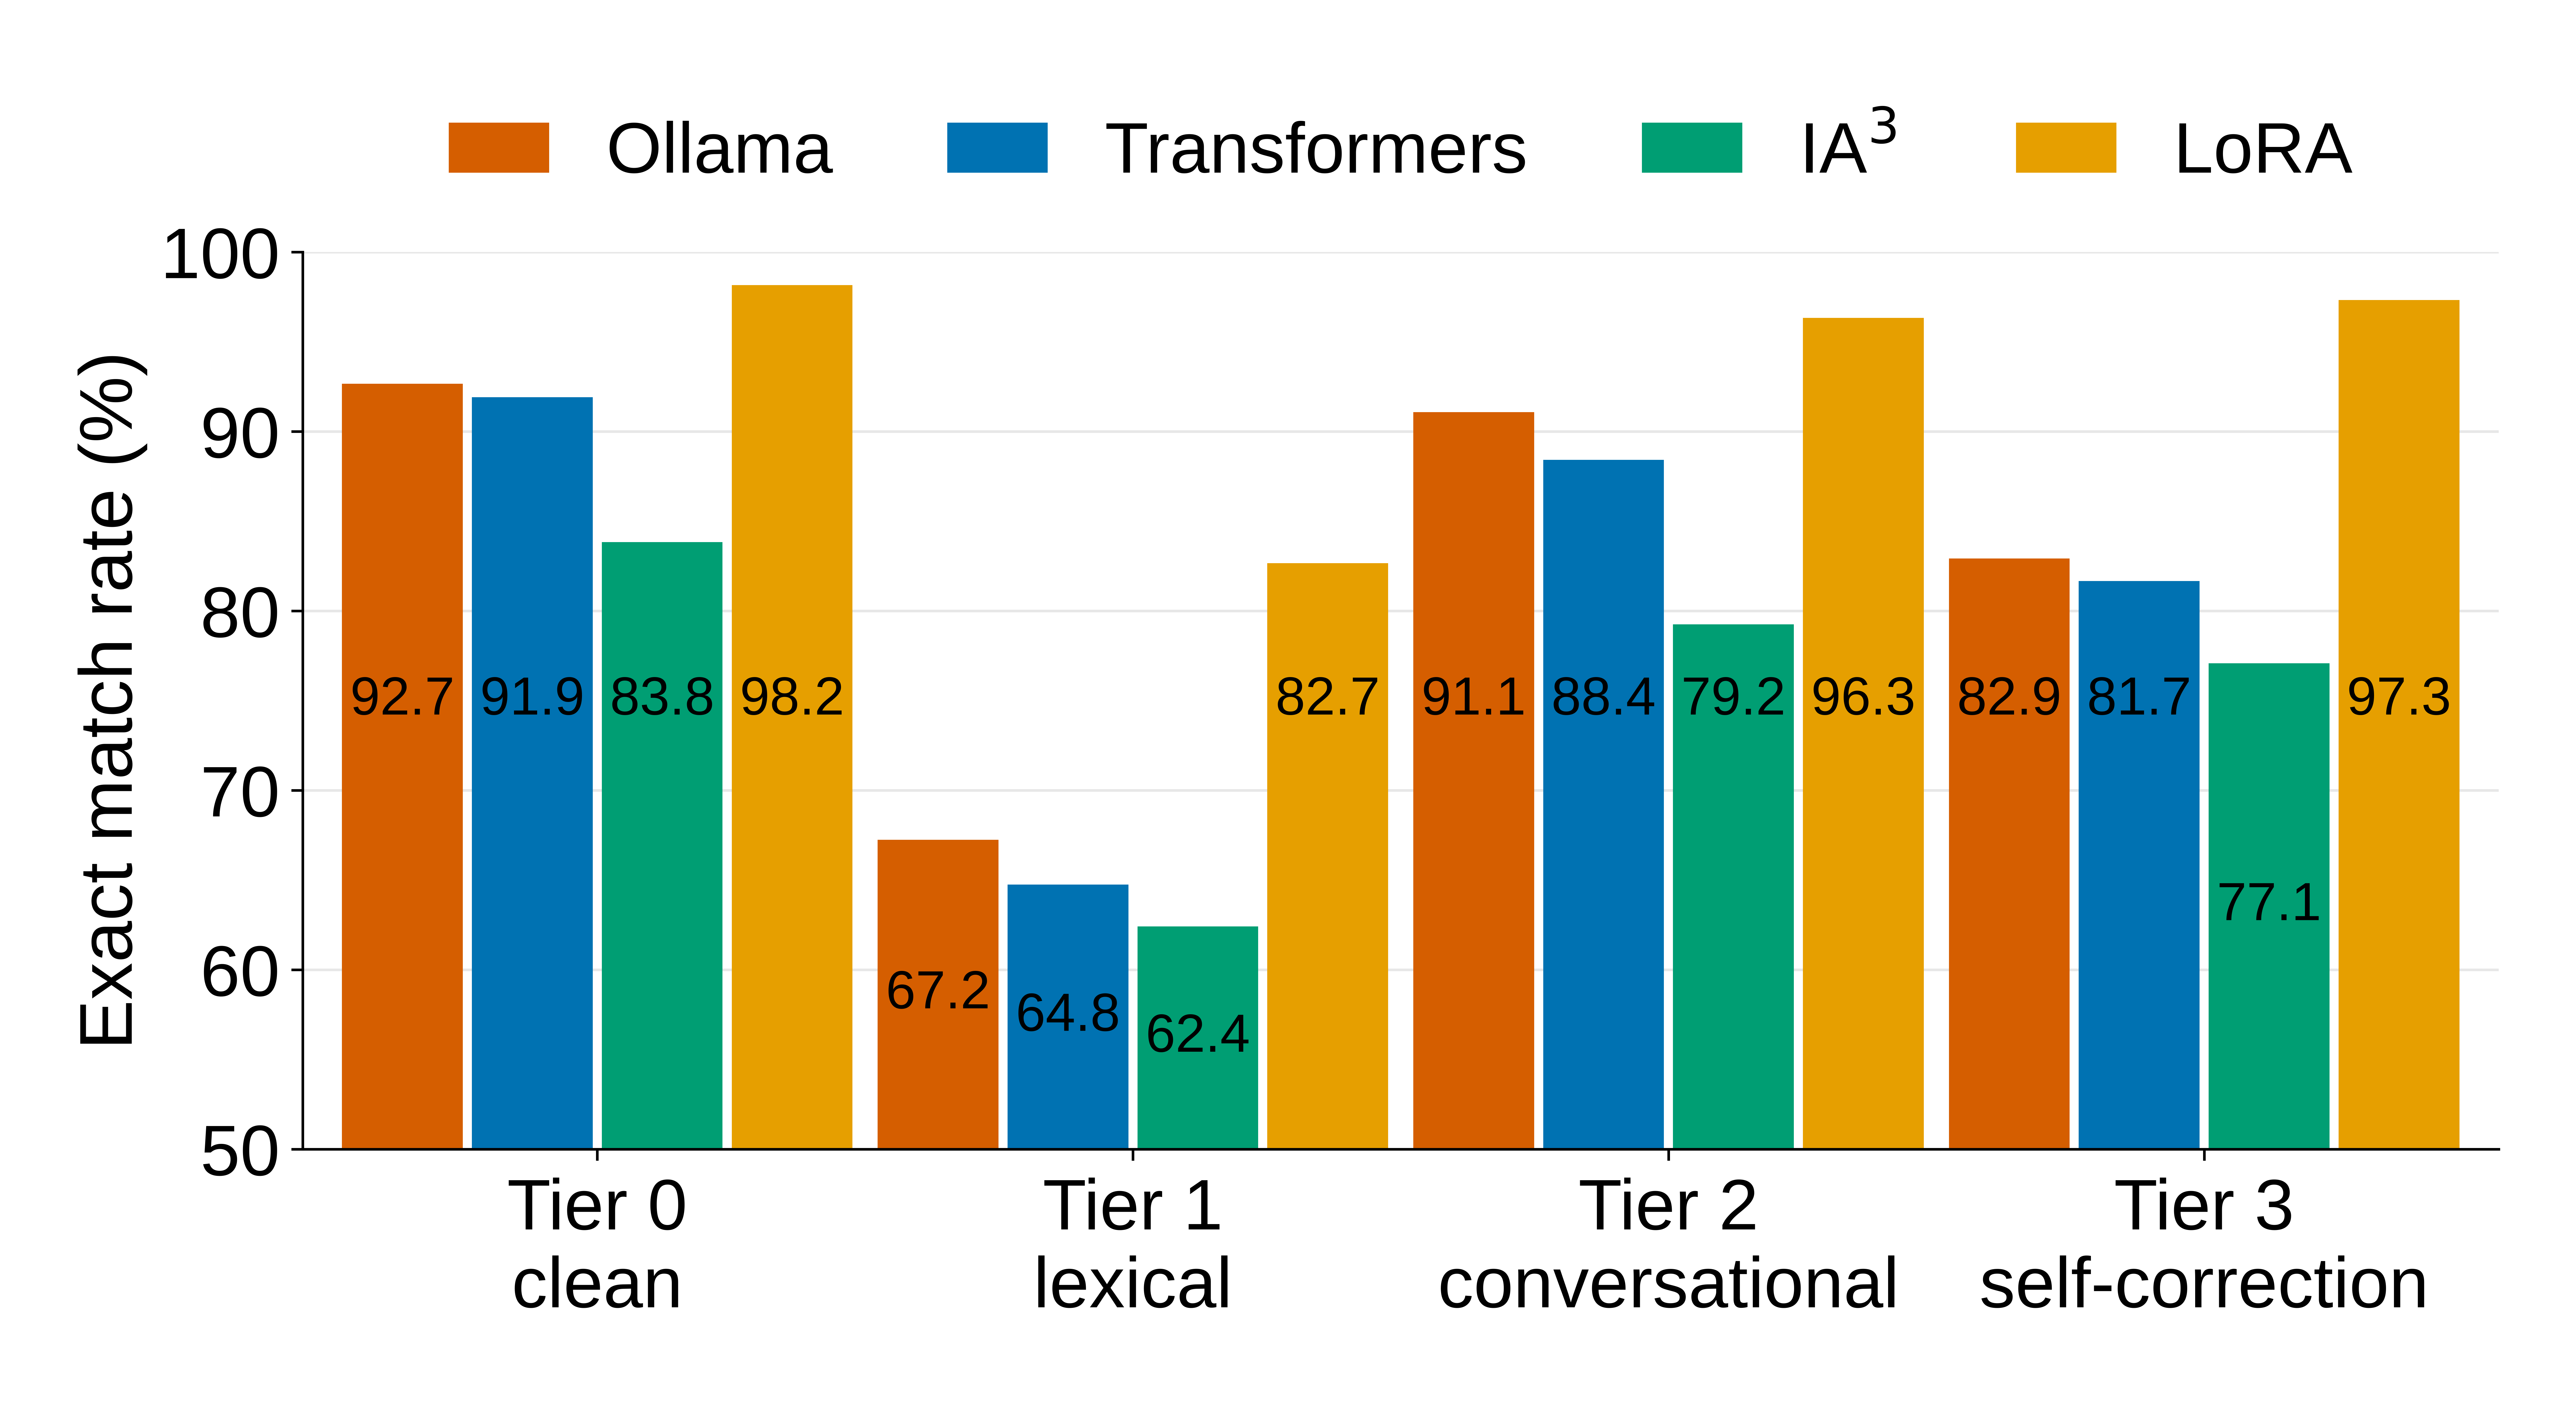
\includegraphics[width=\textwidth]{figures/emr_by_tier_fewshot_3b.png}
\caption{Exact match rate per noise tier for Llama 3.2 3B Instruct with the few-shot prompt. Ollama and Transformers are the two inference setups without adapters; IA$^3$ and LoRA are adapters trained on the 4-bit Transformers base model. Each bar covers 1200 test inputs.\label{fig:emr_tiers_3b}}
\end{figure}

\begin{figure}[H]
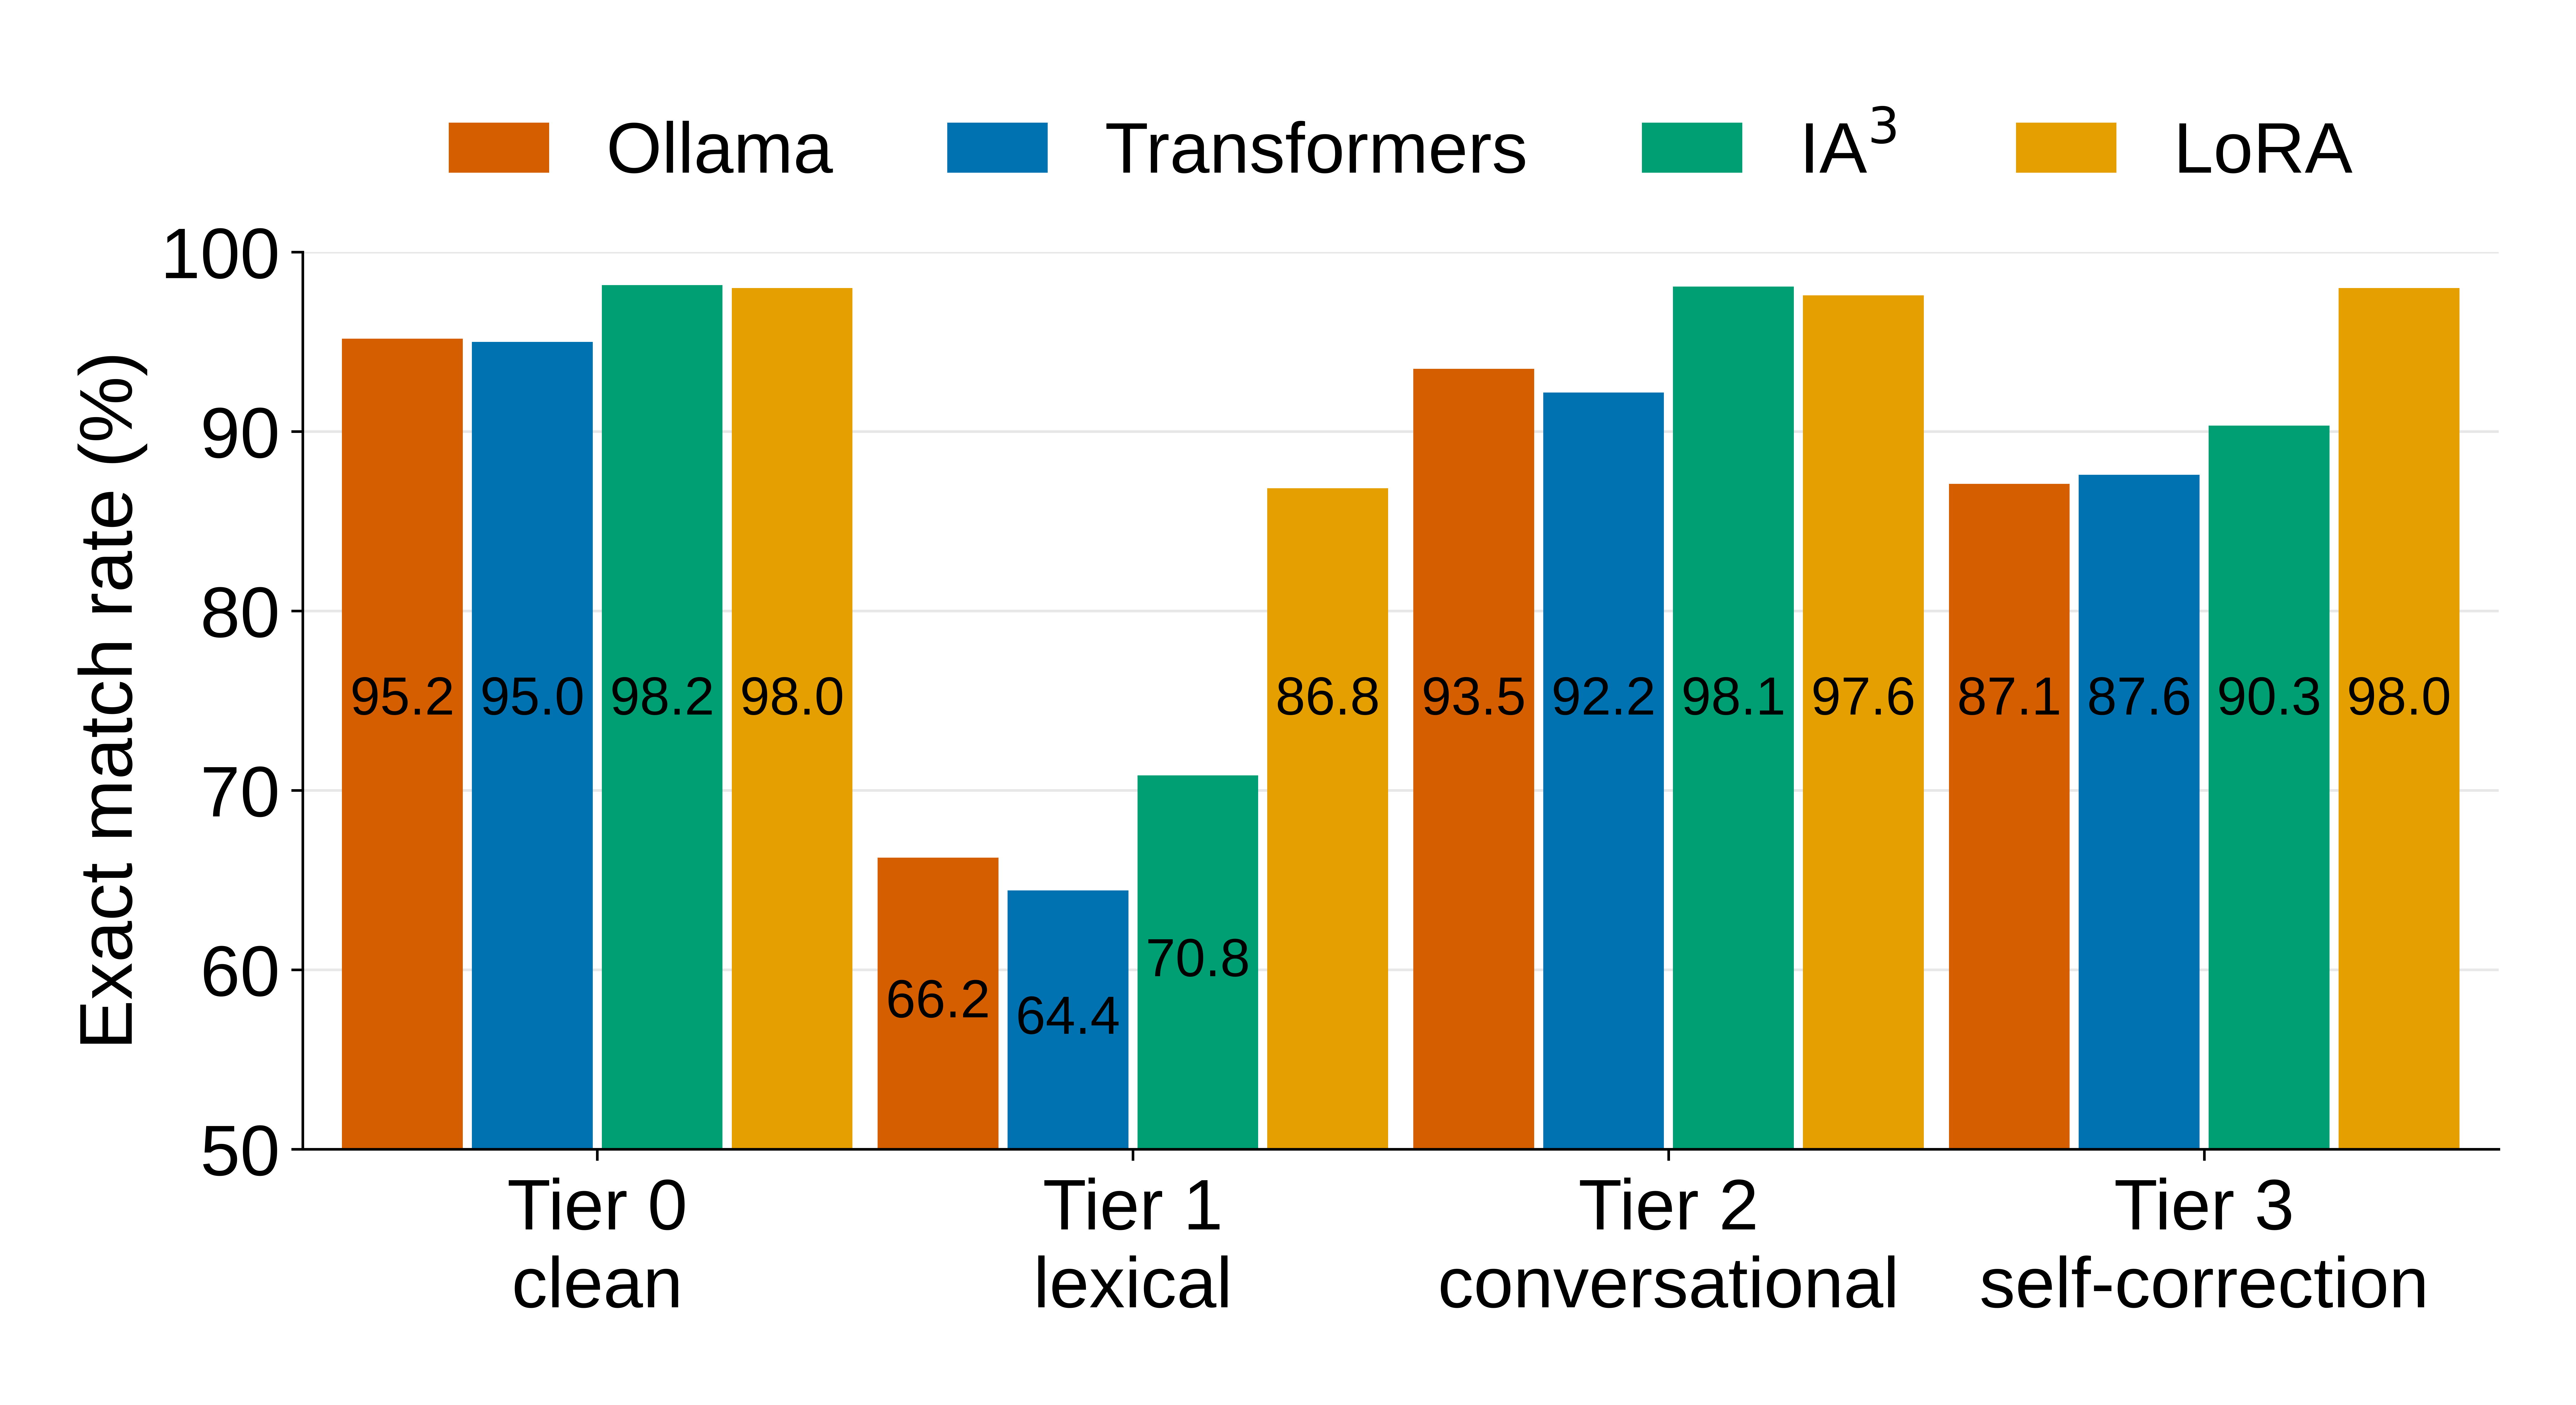
\includegraphics[width=\textwidth]{figures/emr_by_tier_fewshot_8b.png}
\caption{Exact match rate per noise tier for Llama 3.1 8B Instruct with the few-shot prompt. Ollama and Transformers are the two inference setups without adapters; IA$^3$ and LoRA are adapters trained on the 4-bit Transformers base model. Each bar covers 1200 test inputs.\label{fig:emr_tiers_8b}}
\end{figure}

With the extended and few-shot prompts, lexical noise reduced the EMR of both baselines by 25.4 to 30.9 percentage points compared with Tier~0. The drop was 21.4 to 27.6 points for IA$^3$ and 11.2 to 15.5 points for LoRA. The larger model did not reduce this drop: for the baselines, it was 28.9 to 30.9 points with the 8B model and 25.4 to 29.4 points with the 3B model. Conversational noise had a small effect. Tier~2 was at most 6.1 points below Tier~0 for every method with these two prompts. Self-corrections in Tier~3 reduced the EMR of the baselines by 7.4 to 10.3 points with the few-shot prompt and by 24.5 to 36.7 points with the extended prompt. With these two prompts, LoRA was at most 0.8 points below its Tier~0 result on Tier~3.

\subsection{Effect of Prompt Design}\label{sec:res-prompts}

The prompt had a large effect without adapters and almost no effect with LoRA. Figures~\ref{fig:emr_prompts_3b} and~\ref{fig:emr_prompts_8b} show the EMR over all tiers for each prompt. Without adapters, the few-shot prompt was better than the extended prompt in both setups and for both models, by 4.4 to 9.8 points. LoRA stayed between 92.2\% and 93.6\% with the 3B model and between 92.6\% and 95.1\% with the 8B model, whichever prompt it was trained and evaluated with. IA$^3$ depended more on the prompt, with a range of 13.6 points for the 3B model and 9.9 points for the 8B model.

\begin{figure}[H]
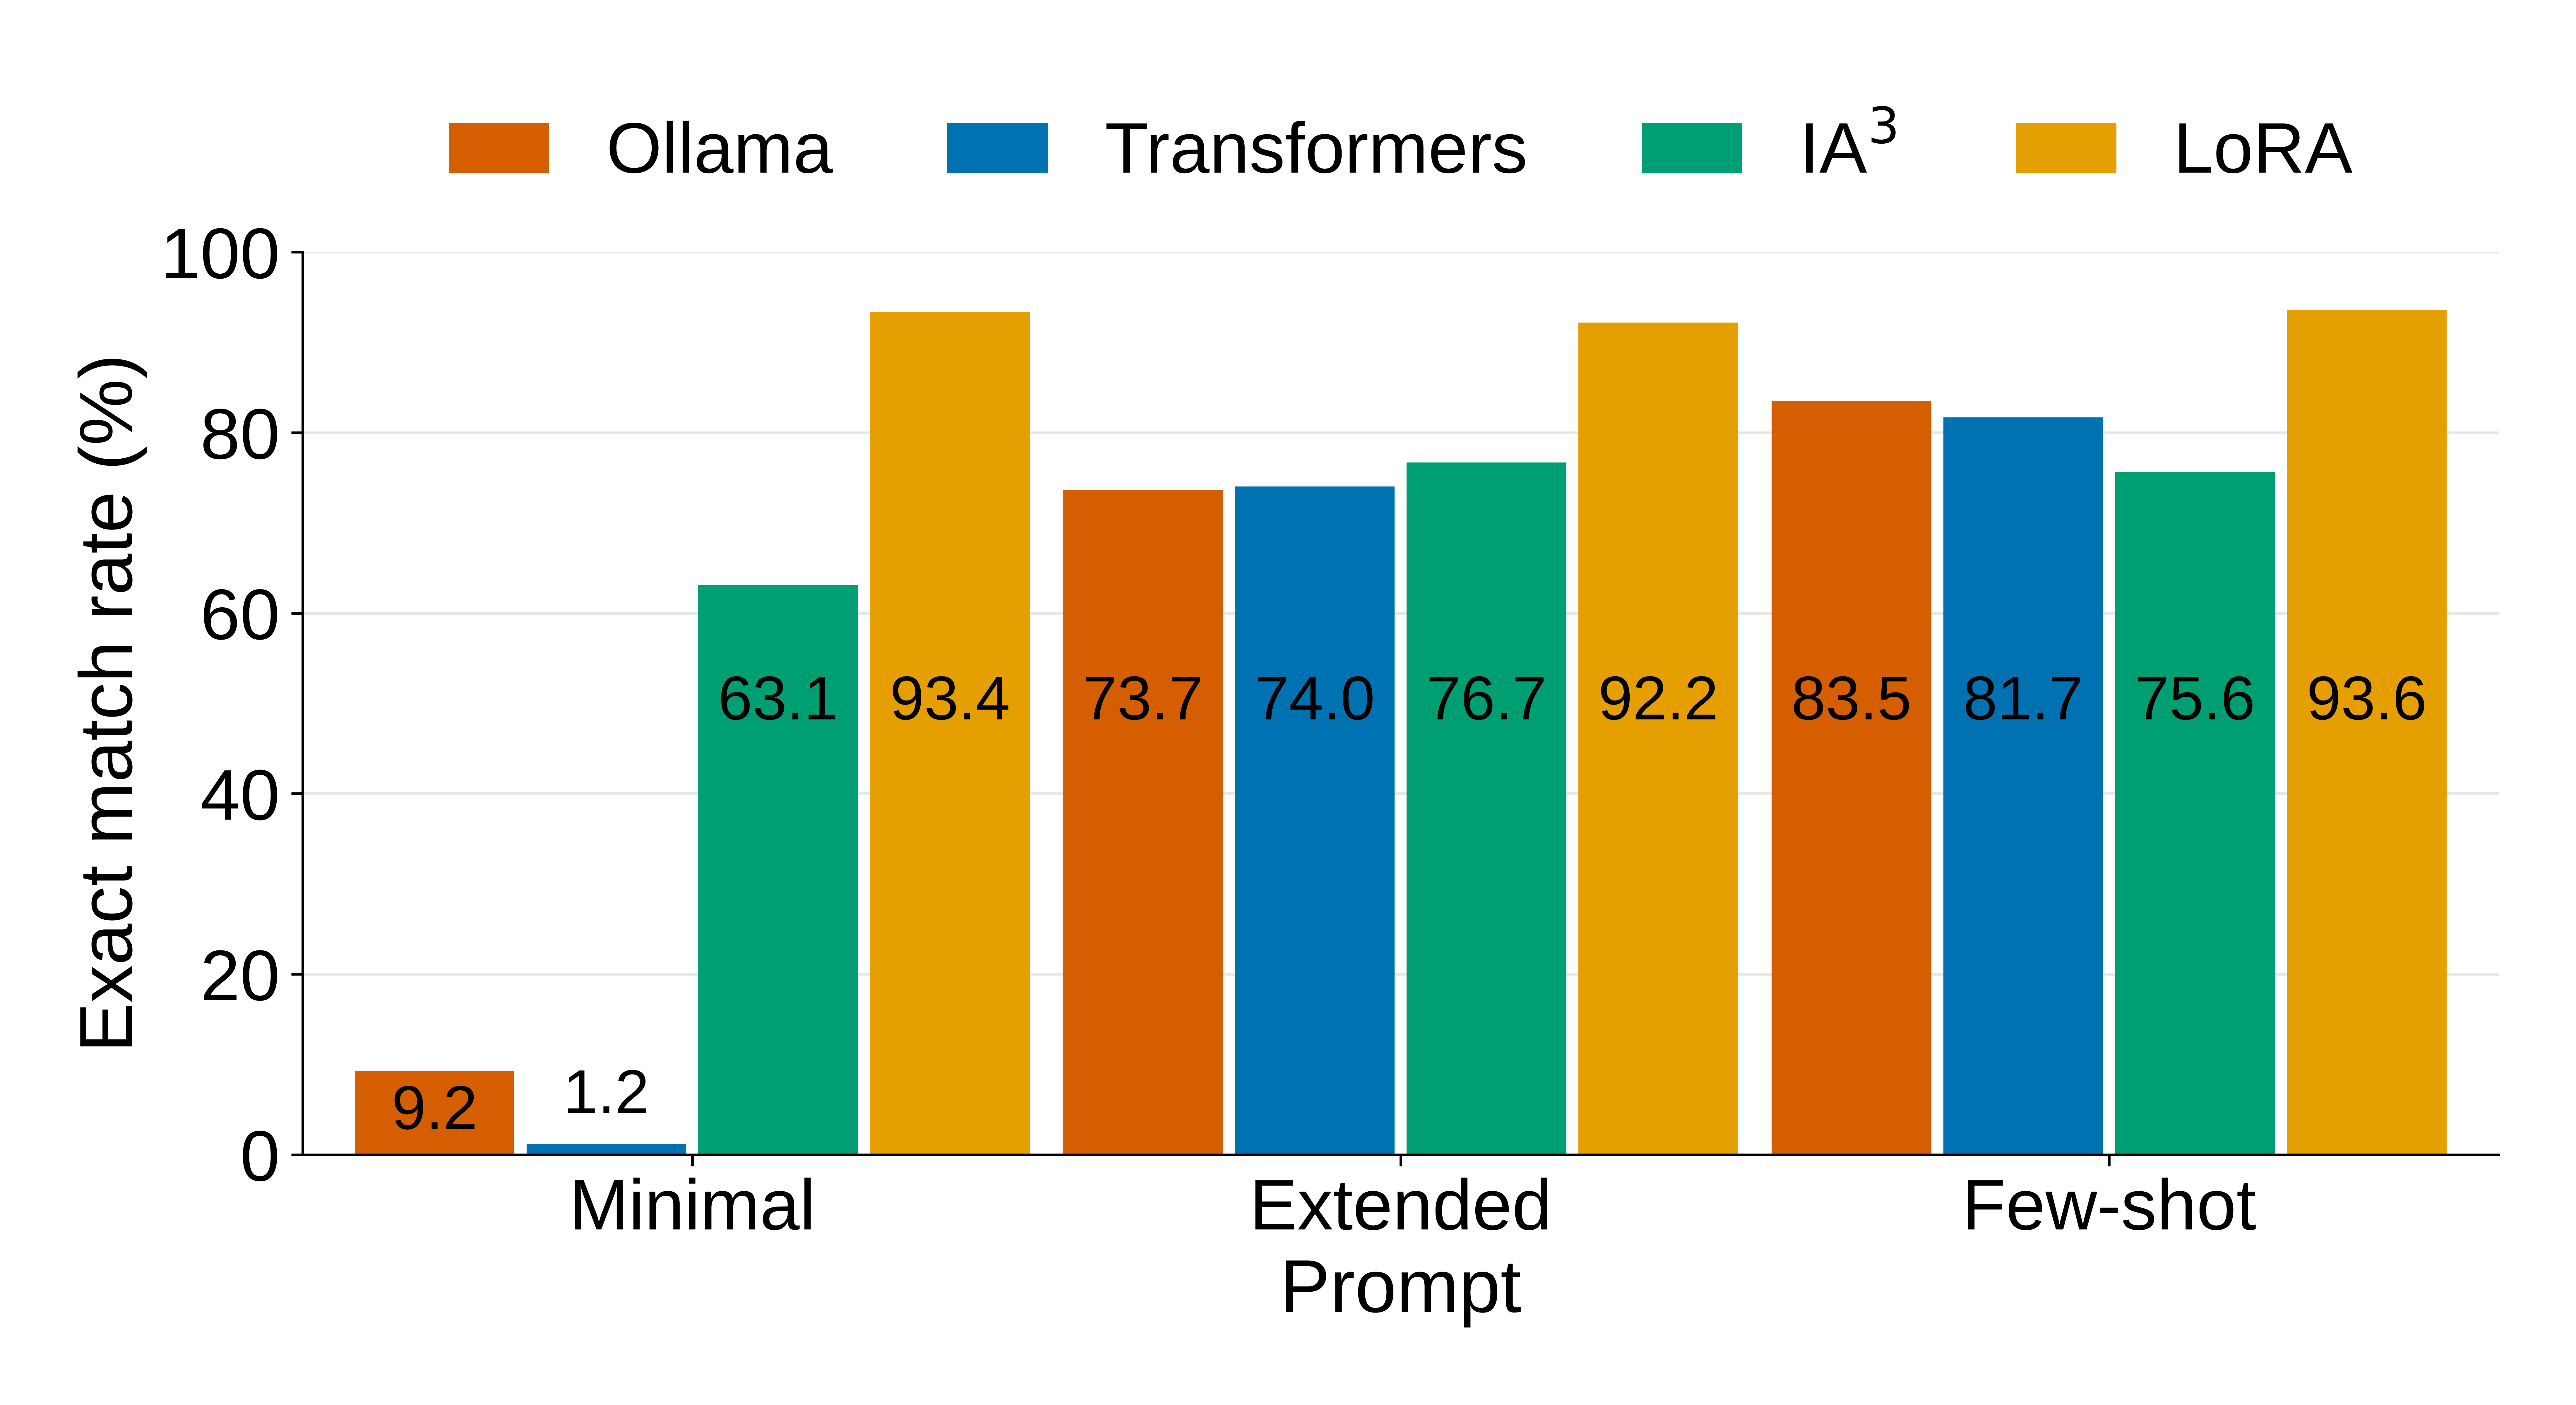
\includegraphics[width=\textwidth]{figures/emr_by_prompt_3b.png}
\caption{Exact match rate over all four tiers (4800 test inputs) for each prompt, Llama 3.2 3B Instruct. Each adapter was trained and evaluated with the same prompt.\label{fig:emr_prompts_3b}}
\end{figure}

\begin{figure}[H]
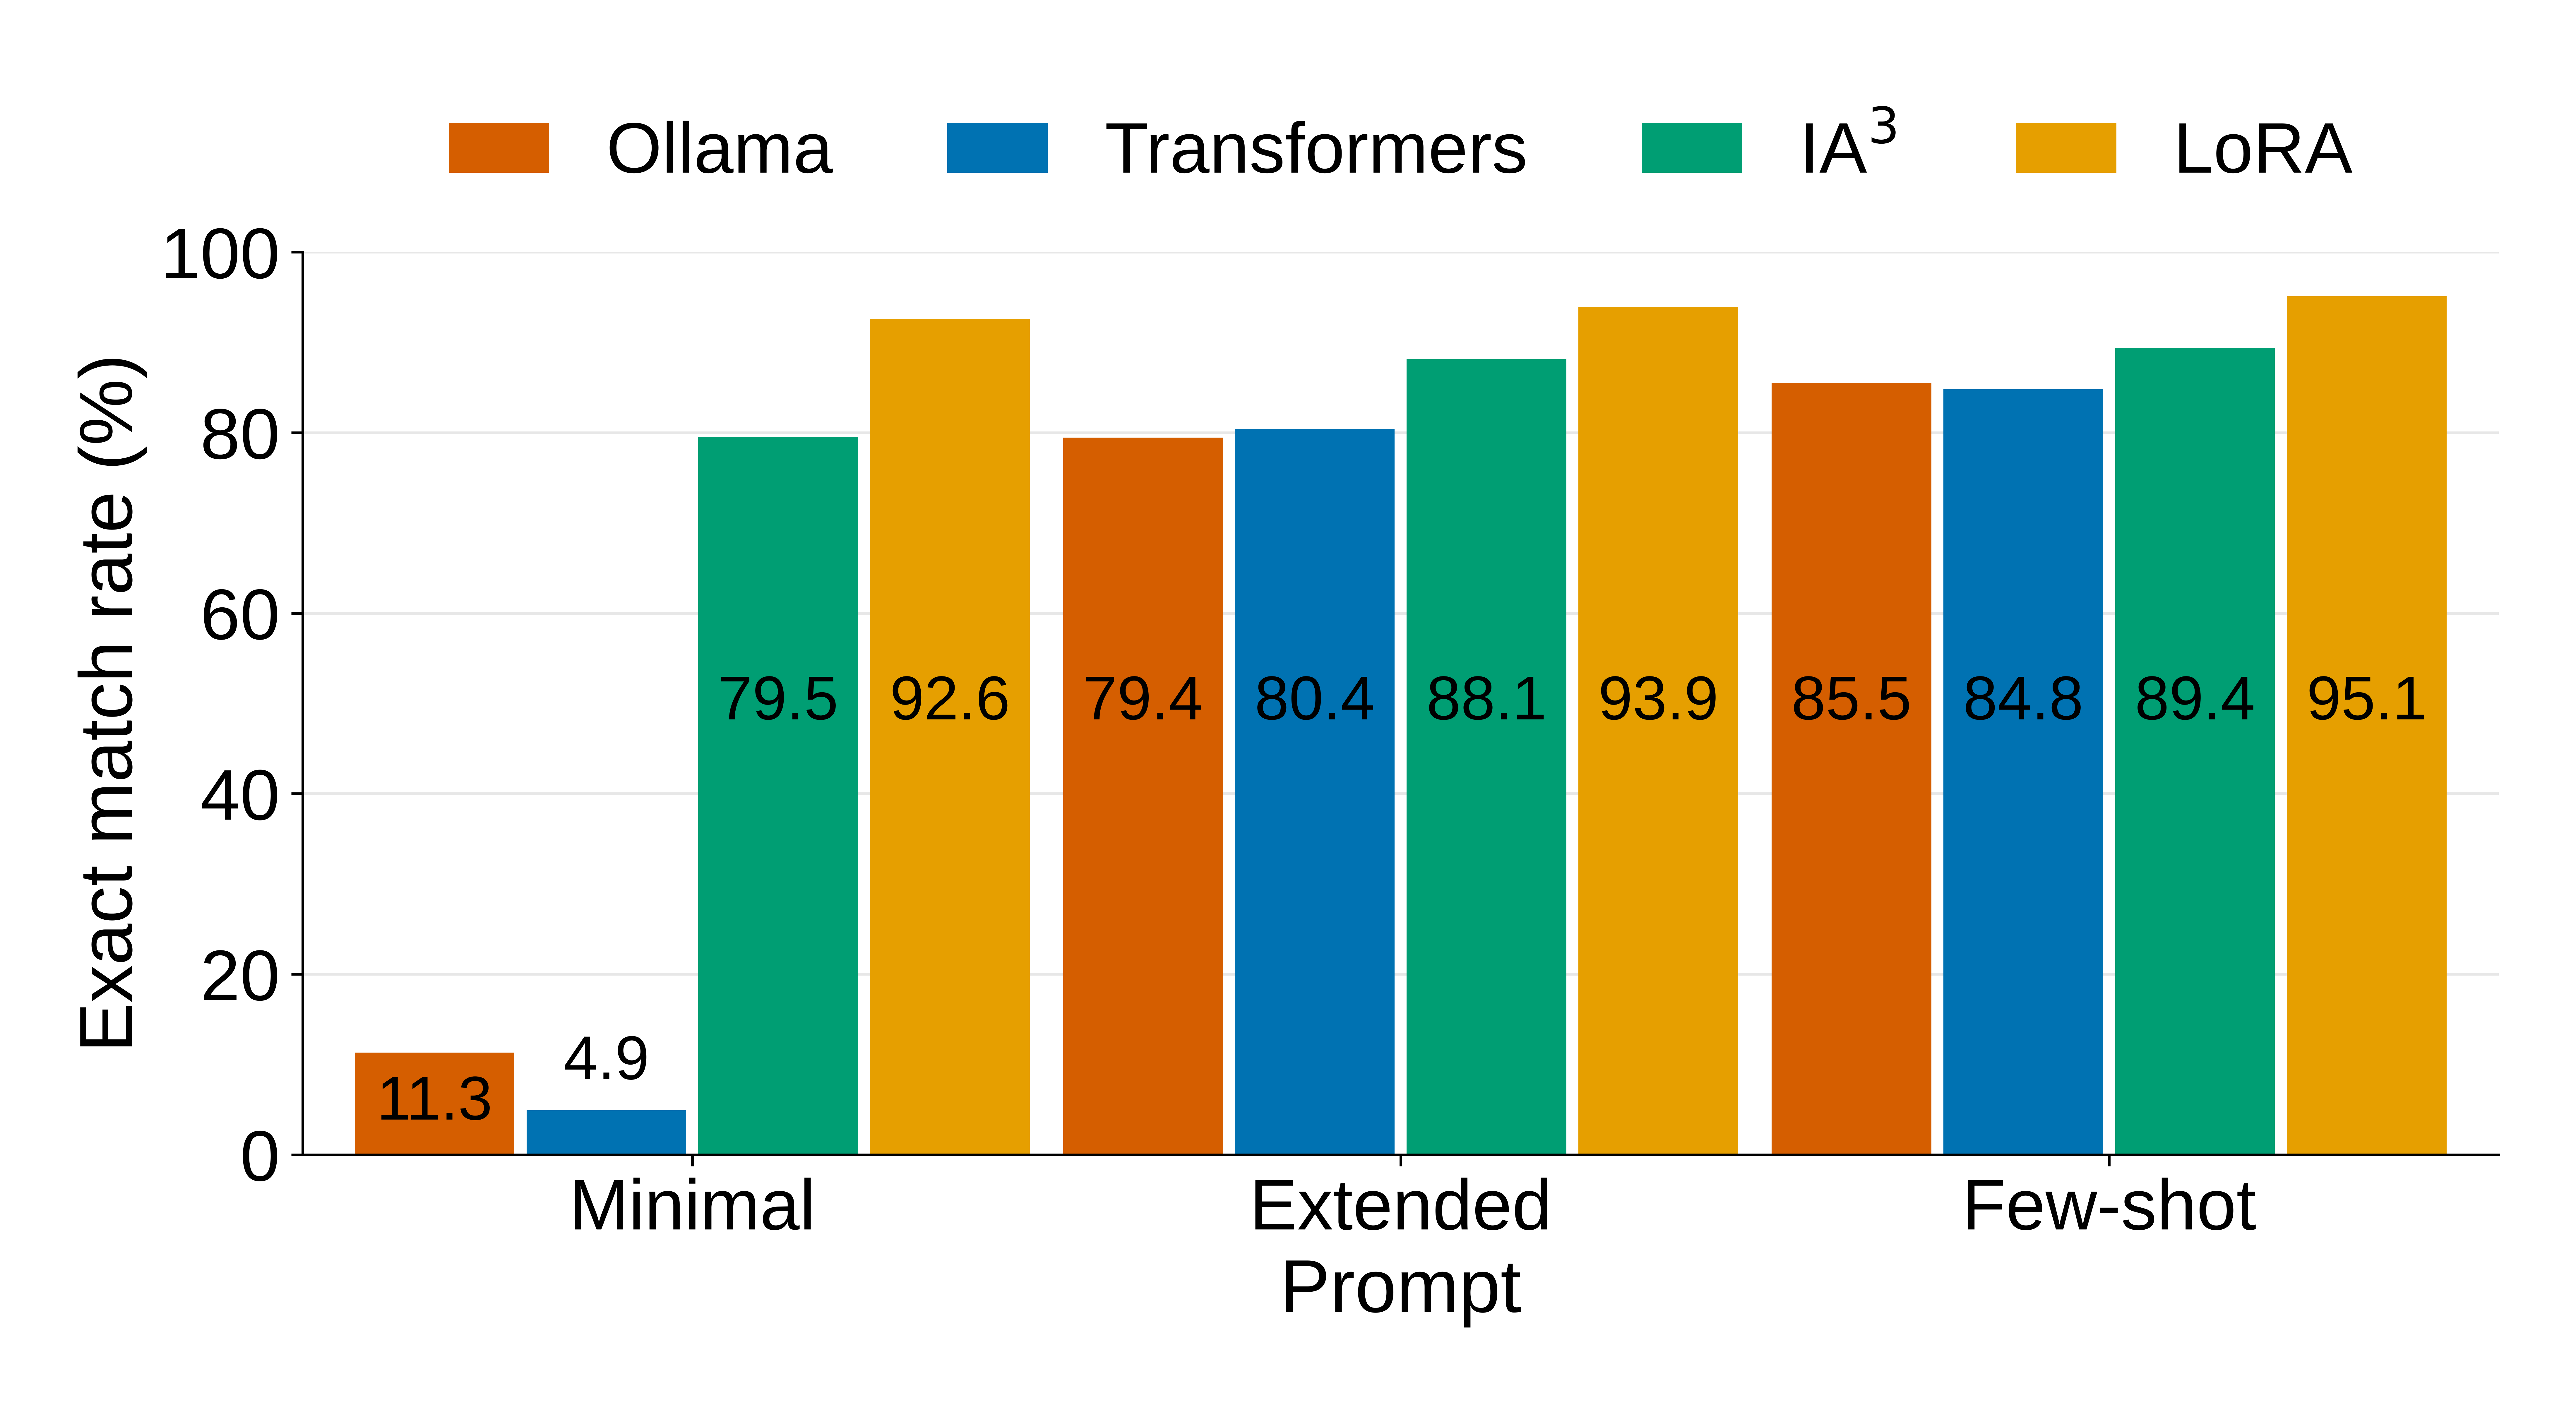
\includegraphics[width=\textwidth]{figures/emr_by_prompt_8b.png}
\caption{Exact match rate over all four tiers (4800 test inputs) for each prompt, Llama 3.1 8B Instruct. Each adapter was trained and evaluated with the same prompt.\label{fig:emr_prompts_8b}}
\end{figure}

With the minimal prompt, both baselines failed, with an EMR of 1.2\% to 11.3\% over all tiers. Table~\ref{tab:minimal} shows that the two setups failed for different reasons. In the Transformers setup, only 29.4\% (3B) and 73.2\% (8B) of the outputs were schema-valid. In the Ollama setup, the JSON schema constraint kept schema adherence at 99.7\% or higher, but only 10.9\% (3B) and 12.5\% (8B) of the outputs used one of the three allowed actions. In 85.2\% (3B) and 73.7\% (8B) of the other outputs, the action field repeated a word or phrase from the command, such as ``return'', ``delete'' or ``grab''. The adapters trained with the minimal prompt did not show this problem: LoRA used an allowed action in 97.7\% (3B) and 99.2\% (8B) of the outputs.

\begin{table}[H]
\caption{Results with the minimal prompt over all 4800 test inputs. Schema adherence is the share of schema-valid outputs. Allowed action is the share of outputs that are schema-valid and whose action is \texttt{add}, \texttt{remove} or \texttt{update}.\label{tab:minimal}}
\begin{tabularx}{\textwidth}{llCCC}
\toprule
Model & Method & Schema adherence (\%) & Allowed action (\%) & EMR (\%) \\
\midrule
3B & Ollama & 99.7 & 10.9 & 9.2 \\
 & Transformers & 29.4 & 1.5 & 1.2 \\
 & IA$^3$ & 95.5 & 89.6 & 63.1 \\
 & LoRA & 100.0 & 97.7 & 93.4 \\
\midrule
8B & Ollama & 100.0 & 12.5 & 11.3 \\
 & Transformers & 73.2 & 5.6 & 4.9 \\
 & IA$^3$ & 98.8 & 90.9 & 79.5 \\
 & LoRA & 100.0 & 99.2 & 92.6 \\
\bottomrule
\end{tabularx}
\end{table}

\subsection{Error Analysis}\label{sec:res-errors}

To see where the methods fail, we examined field accuracy on Tier~1 and the action errors on Tier~3. Figure~\ref{fig:fields_tier1_8b} shows the field accuracy on Tier~1 for the 8B model with the few-shot prompt. The product was the least accurate field for every method. Without adapters and with IA$^3$, between 71.9\% and 75.2\% of the products were correct, compared with 89.1\% for LoRA. Action and quantity accuracy were between 88.3\% and 99.0\% for all methods. The 3B model showed the same order, with product accuracy between 74.8\% and 86.8\%. One difference was that 3B IA$^3$ had a lower action accuracy (81.1\%) than both baselines (91.1\% in the Ollama setup and 87.1\% in the Transformers setup).

\begin{figure}[H]
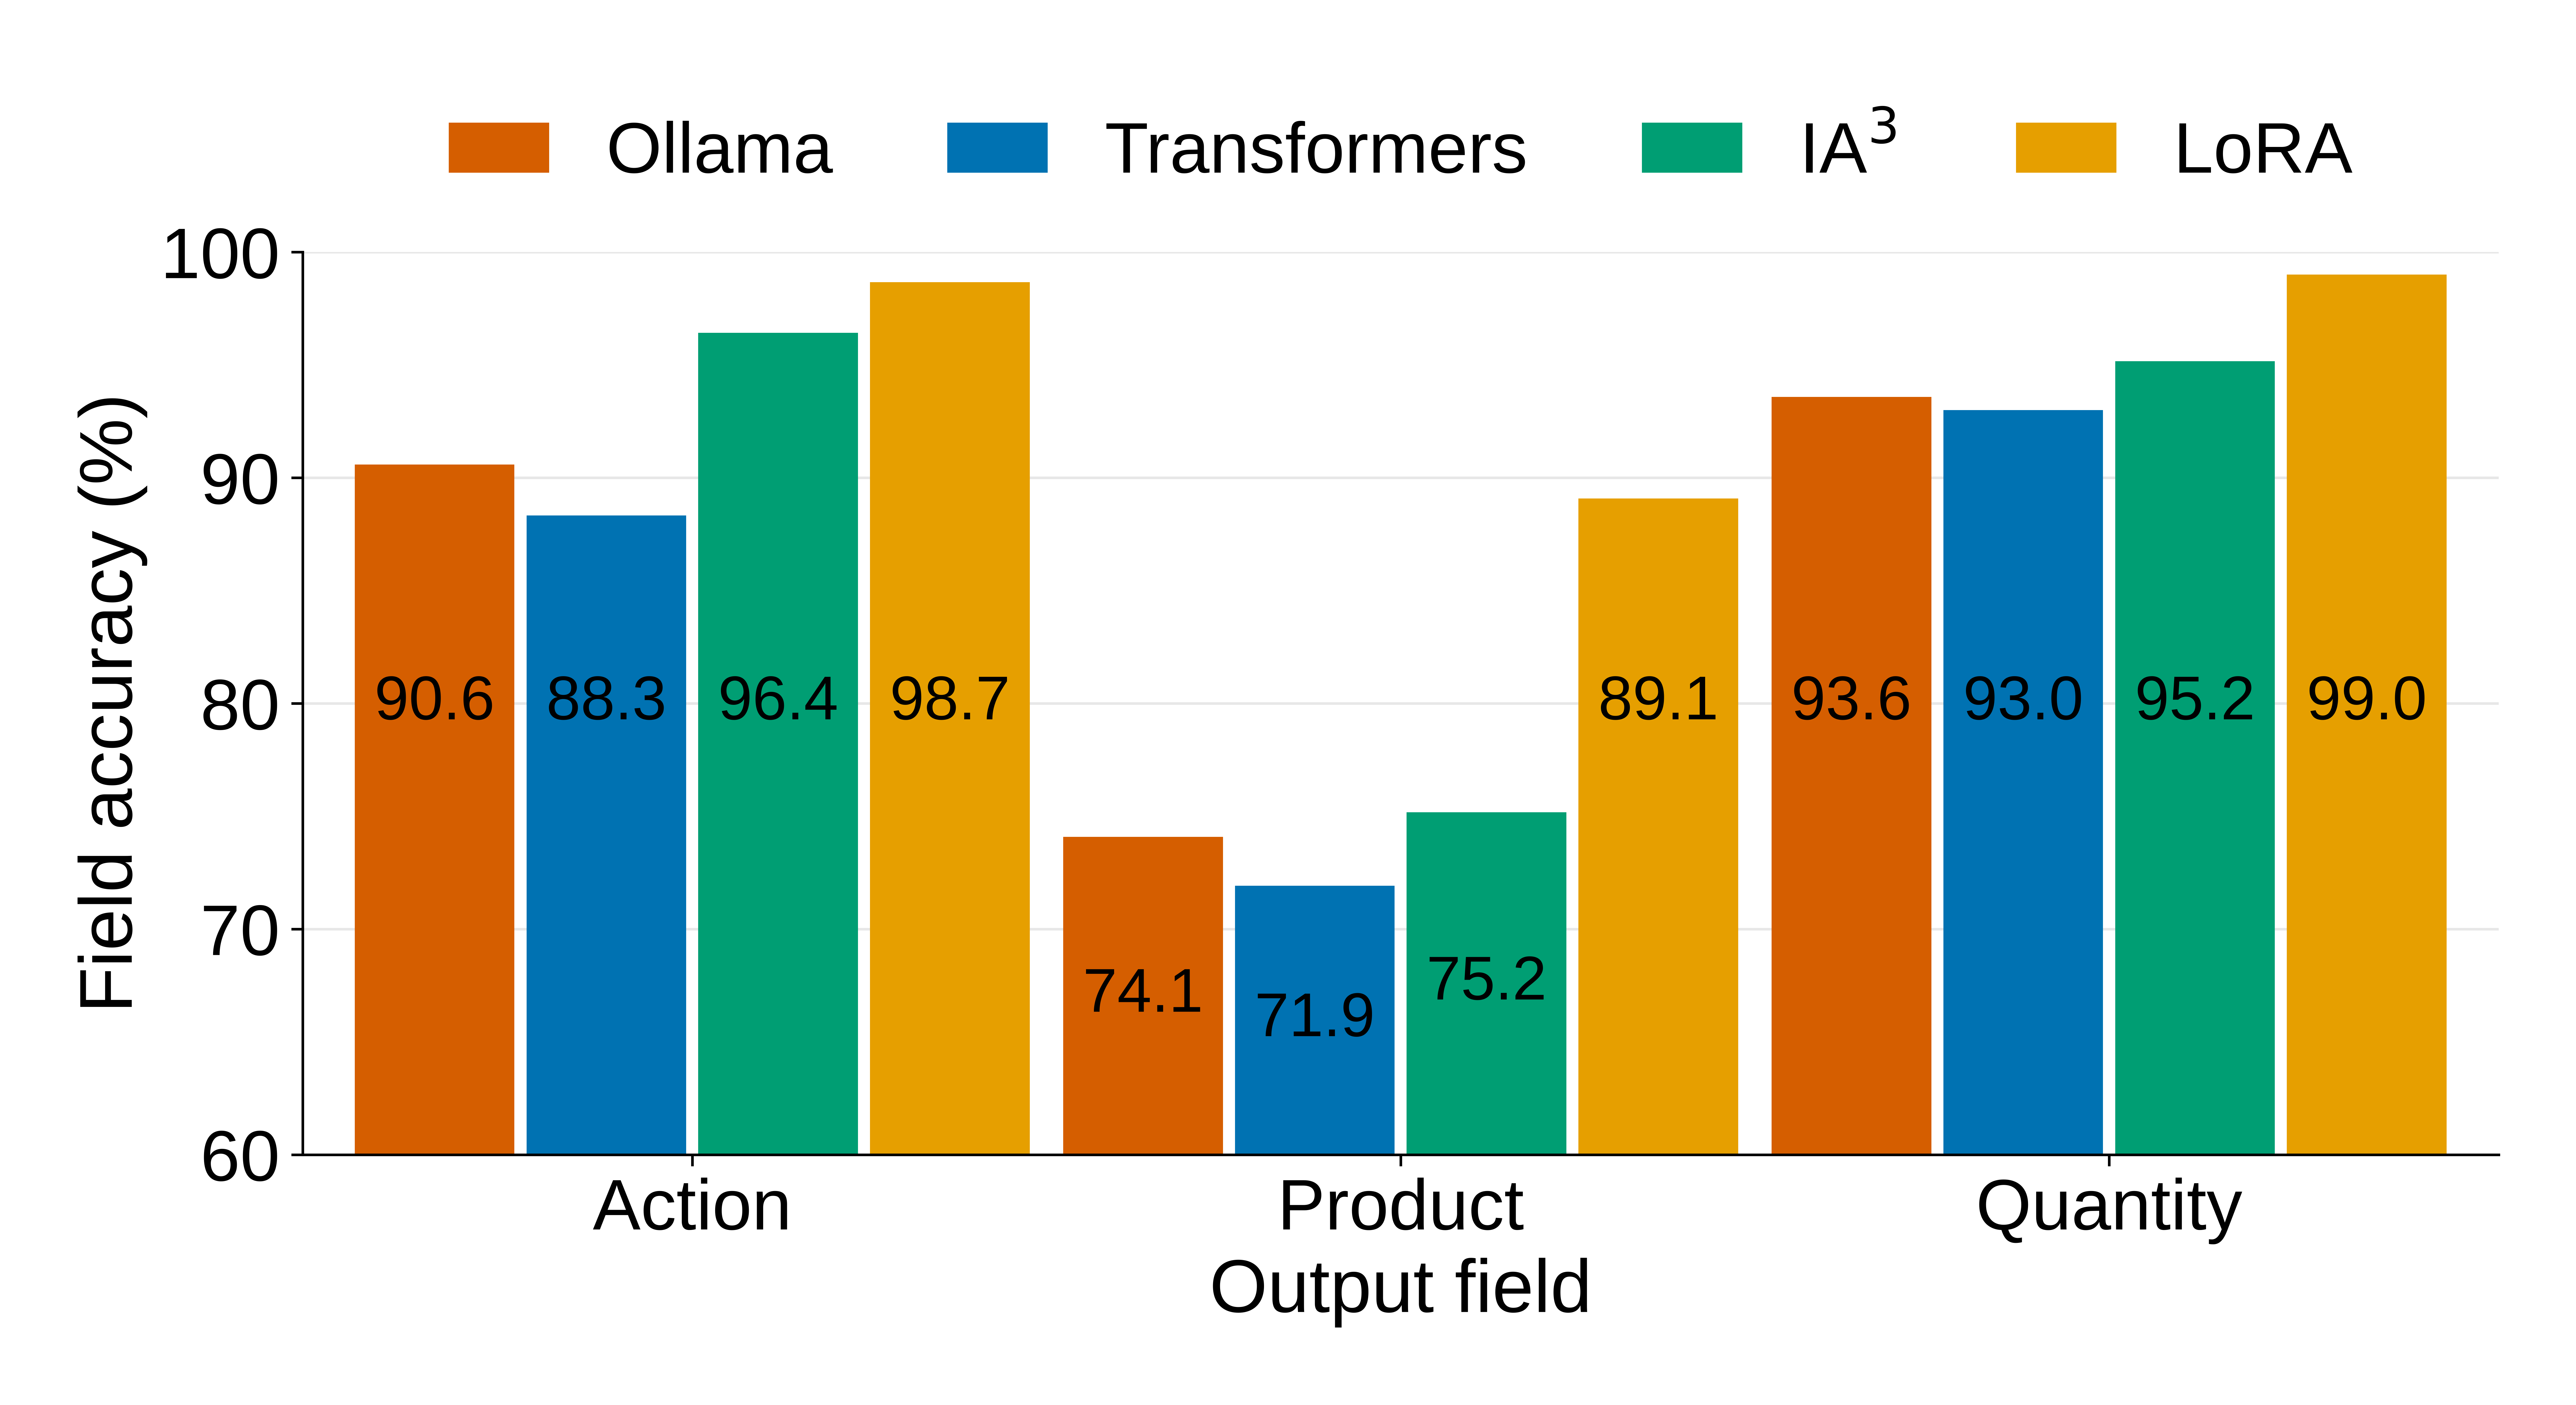
\includegraphics[width=\textwidth]{figures/field_accuracy_tier1_8b.png}
\caption{Field accuracy on Tier~1 (lexical noise, 1200 inputs) for Llama 3.1 8B Instruct with the few-shot prompt. A field counts as correct only if the output is schema-valid and the field equals the reference after lowercasing and whitespace normalization.\label{fig:fields_tier1_8b}}
\end{figure}

The product errors on Tier~1 differed in type between methods. In 325 of the 1200 Tier~1 commands, the product name itself contains a vowel deletion. With the few-shot prompt, 87.9\% to 95.9\% of the wrong products in schema-valid outputs of the baselines, and 77.1\% to 93.8\% of those of IA$^3$, appeared verbatim in the noisy command. For example, both baselines returned ``mnt laves'' for ``mint leaves''. LoRA copied the command text in only 13.9\% (3B) and 16.8\% (8B) of its product errors. Its other product errors replaced the noisy name with a different product, such as ``mozzarella'' for ``mnt laves'' or ``termite'' for ``trmrc'' (turmeric), or changed the number of the noun, such as ``mop head'' for ``mop hds'' (mop heads).

On Tier~3, most errors were wrong actions. Table~\ref{tab:tier3} counts these errors for the extended and few-shot prompts. With the extended prompt, the Ollama and Transformers baselines returned a wrong action for 302 to 445 of the 1200 Tier~3 inputs. In 259 to 422 of these cases, the model labeled an \texttt{add} or \texttt{remove} command as \texttt{update}. With the few-shot prompt, the number of such \texttt{update} labels fell to between 20 and 126. With these two prompts, LoRA returned at most 35 wrong actions and at most 3 such \texttt{update} labels. IA$^3$ with the 3B model and the extended prompt made 241 action errors of another kind: most of them labeled \texttt{update} commands as \texttt{add} or \texttt{remove}, or \texttt{remove} commands as \texttt{add}.

\begin{table}[H]
\caption{Errors on Tier~3 (self-correction, 1200 inputs) with the extended and few-shot prompts. Errors are inputs without an exact match. Wrong action counts schema-valid outputs with an incorrect action. Add or remove labeled as update counts outputs that return \texttt{update} for a command whose correct action is \texttt{add} or \texttt{remove}.\label{tab:tier3}}
\begin{tabularx}{\textwidth}{lllCCC}
\toprule
Model & Prompt & Method & Errors & Wrong action & Add or remove labeled as update \\
\midrule
3B & Extended & Ollama & 492 & 440 & 417 \\
 &  & Transformers & 440 & 392 & 348 \\
 &  & IA$^3$ & 273 & 241 & 3 \\
 &  & LoRA & 64 & 35 & 3 \\
\midrule
 & Few-shot & Ollama & 205 & 175 & 106 \\
 &  & Transformers & 220 & 196 & 126 \\
 &  & IA$^3$ & 275 & 248 & 95 \\
 &  & LoRA & 32 & 21 & 0 \\
\midrule
8B & Extended & Ollama & 483 & 445 & 422 \\
 &  & Transformers & 356 & 302 & 259 \\
 &  & IA$^3$ & 158 & 111 & 71 \\
 &  & LoRA & 44 & 6 & 0 \\
\midrule
 & Few-shot & Ollama & 155 & 143 & 47 \\
 &  & Transformers & 149 & 94 & 20 \\
 &  & IA$^3$ & 116 & 93 & 65 \\
 &  & LoRA & 24 & 4 & 0 \\
\bottomrule
\end{tabularx}
\end{table}

\subsection{Statistical Comparisons}\label{sec:res-stats}

The McNemar tests confirmed most of the differences described above. Table~\ref{tab:mcnemar} summarizes the 96 tests. LoRA was significantly better than the Transformers baseline in 23 of 24 comparisons. The exception was the 8B model with the extended prompt on Tier~0, where the difference was 1.3 points. With the few-shot prompt, LoRA improved the EMR by 6.3 to 17.9 points for the 3B model and by 3.0 to 22.4 points for the 8B model, with the largest gains on Tier~1.

\begin{table}[H]
\caption{Summary of the exact McNemar tests on EMR. Each row covers 12 tests (three prompts and four tiers). A difference counts as significant if its Holm-corrected $p$-value over all 96 tests is below 0.05.\label{tab:mcnemar}}
\begin{tabularx}{\textwidth}{llCCC}
\toprule
Comparison (A vs. B) & Model & A significantly better & B significantly better & No significant difference \\
\midrule
LoRA vs. Transformers & 3B & 12 & 0 & 0 \\
 & 8B & 11 & 0 & 1 \\
\midrule
IA$^3$ vs. Transformers & 3B & 5 & 4 & 3 \\
 & 8B & 11 & 0 & 1 \\
\midrule
LoRA vs. IA$^3$ & 3B & 12 & 0 & 0 \\
 & 8B & 8 & 0 & 4 \\
\midrule
Ollama vs. Transformers & 3B & 5 & 1 & 6 \\
 & 8B & 6 & 1 & 5 \\
\bottomrule
\end{tabularx}
\end{table}

The effect of IA$^3$ depended on the model size. With the 8B model, IA$^3$ was significantly better than the Transformers baseline in 11 of 12 comparisons. With the 3B model, it was better with the minimal prompt and on Tier~3 with the extended prompt (by 13.9 points), but significantly worse in four comparisons: on Tiers~0, 2 and~3 with the few-shot prompt (by 8.1, 9.2 and 4.6 points) and on Tier~2 with the extended prompt (by 4.3 points). LoRA was significantly better than IA$^3$ in all 12 comparisons with the 3B model. With the 8B model, the two adapters did not differ significantly on Tiers~0 and~2 with the extended and few-shot prompts, where the differences were at most 1.1 points, while LoRA was better on Tiers~1 and~3 by 7.7 to 16.0 points.

The two setups without adapters differed mainly with the minimal prompt, where the Ollama setup was significantly better on all eight model and tier combinations, by 4.0 to 9.8 points. With the extended prompt, the Transformers setup was significantly better on Tier~3, by 4.3 points (3B) and 10.6 points (8B). The Ollama setup was also better on Tiers~1 and~2 with the 8B model and the extended prompt, by 2.6 and 3.6 points. With the few-shot prompt, only one of eight comparisons was significant: the Ollama setup was 2.7 points better on Tier~2 with the 3B model.

\subsection{Training and Inference Cost}\label{sec:res-cost}

The adapters add a one-time training cost, and they also change the cost of each prediction. Table~\ref{tab:training} lists the training time and the peak GPU memory during training. Training one LoRA adapter took 11.5 to 11.6 hours for the 3B model and 13.3 to 13.4 hours for the 8B model, which is 26\% to 32\% longer than training the IA$^3$ adapter for the same model and prompt. Peak memory was almost the same for the two adapter types but grew with the prompt length, from 3.9~GB with the minimal prompt to 8.3~GB with the few-shot prompt for the 3B model, and from 13.0~GB to 18.1~GB for the 8B model. Training energy was not measured.

\begin{table}[H]
\caption{Adapter training cost. Each adapter was trained for three epochs on 38,400 training examples on a single NVIDIA A100 GPU with 40~GB of memory. Peak memory is the maximum GPU memory allocated during training.\label{tab:training}}
\begin{tabularx}{\textwidth}{lllCC}
\toprule
Model & Adapter & Prompt & Training time (h) & Peak memory (GB) \\
\midrule
3B & IA$^3$ & Minimal & 9.1 & 3.9 \\
 &  & Extended & 8.8 & 5.9 \\
 &  & Few-shot & 9.1 & 8.2 \\
\midrule
 & LoRA & Minimal & 11.5 & 3.9 \\
 &  & Extended & 11.6 & 5.9 \\
 &  & Few-shot & 11.5 & 8.3 \\
\midrule
8B & IA$^3$ & Minimal & 10.6 & 13.0 \\
 &  & Extended & 10.5 & 15.3 \\
 &  & Few-shot & 10.5 & 18.1 \\
\midrule
 & LoRA & Minimal & 13.3 & 13.1 \\
 &  & Extended & 13.3 & 15.3 \\
 &  & Few-shot & 13.4 & 18.1 \\
\bottomrule
\end{tabularx}
\end{table}

Table~\ref{tab:efficiency} lists the inference energy and speed. The Ollama setup used 18.9 to 38.4~Wh per 1000 inputs, which is 2.5 to 3.9 times less than the Transformers setup with the same model and prompt (63.5 to 114.2~Wh). Compared with the Transformers baseline, LoRA used between 4\% less and 45\% more energy per input, depending on the model and prompt; the largest increase was with the 3B model and the few-shot prompt (91.8 compared with 63.5~Wh). IA$^3$ used between 73.1 and 96.6~Wh per 1000 inputs. In the Transformers setup, generation speed was 19.1 to 22.8 tokens per second without adapters, 15.0 to 17.8 with IA$^3$ and 12.1 to 14.4 with LoRA.

\begin{table}[H]
\caption{Inference cost on the 4800 test inputs. Energy is the GPU, CPU and memory energy measured by CodeCarbon, given per 1000 inputs. Speed is output tokens per second, averaged over the four tiers; Ollama speed excludes input processing, so it is not comparable with the other three methods (Section~\ref{sec:efficiency}).\label{tab:efficiency}}
\begin{tabularx}{\textwidth}{lllCC}
\toprule
Model & Prompt & Method & Energy per 1000 inputs (Wh) & Speed (tokens/s) \\
\midrule
3B & Minimal & Ollama & 21.2 & 191.0 \\
 &  & Transformers & 82.1 & 22.8 \\
 &  & IA$^3$ & 73.1 & 17.8 \\
 &  & LoRA & 87.9 & 14.4 \\
\midrule
 & Extended & Ollama & 22.2 & 220.5 \\
 &  & Transformers & 81.0 & 22.0 \\
 &  & IA$^3$ & 77.5 & 16.8 \\
 &  & LoRA & 91.5 & 14.0 \\
\midrule
 & Few-shot & Ollama & 18.9 & 206.7 \\
 &  & Transformers & 63.5 & 21.8 \\
 &  & IA$^3$ & 76.4 & 16.9 \\
 &  & LoRA & 91.8 & 14.0 \\
\midrule
8B & Minimal & Ollama & 35.1 & 144.3 \\
 &  & Transformers & 114.2 & 19.3 \\
 &  & IA$^3$ & 91.7 & 15.0 \\
 &  & LoRA & 109.1 & 12.2 \\
\midrule
 & Extended & Ollama & 38.4 & 147.4 \\
 &  & Transformers & 106.3 & 19.2 \\
 &  & IA$^3$ & 94.3 & 15.0 \\
 &  & LoRA & 113.6 & 12.2 \\
\midrule
 & Few-shot & Ollama & 36.5 & 148.8 \\
 &  & Transformers & 91.1 & 19.1 \\
 &  & IA$^3$ & 96.6 & 15.1 \\
 &  & LoRA & 118.3 & 12.1 \\
\bottomrule
\end{tabularx}
\end{table}

\subsection{Reproducibility}\label{sec:res-repro}

The two complete evaluation runs gave almost the same results. All outputs were identical between the runs for every configuration in the Ollama setup and for every configuration with the 8B model. With the 3B model, the Transformers baseline, IA$^3$ and LoRA were not fully deterministic: between 8 and 584 of the 4800 raw outputs per configuration differed between the runs. The EMR of any tier changed by at most 1.17 percentage points. Of the 96 McNemar tests, 95 gave the same decision in both runs. The exception was the comparison of the two setups for the 3B model with the few-shot prompt on Tier~1, which was significant in the first run (3.3 points, corrected $p = 0.005$) but not in the second (2.5 points, corrected $p = 0.092$). We therefore do not treat this difference as reliable.

\subsection{Discussion}\label{sec:discussion}

This subsection answers the four research questions and relates the results to prior work. Each answer is limited to the two Llama models, the retail-cart task and the test set used here.

RQ1 asked how much each type of noise reduces accuracy without fine-tuning. Lexical noise had by far the largest effect, reducing the EMR of both baselines by 25 to 31 points with the two better prompts, while conversational noise cost at most about 6 points. The size of the drop did not shrink with the larger model, and the field analysis points to the reason: most wrong products were copied from the noisy command. Without fine-tuning, the models extracted the product span as written, but the reference requires its correct spelling. The effect of self-corrections depended mainly on the prompt. With the extended prompt, many corrected commands were labeled as \texttt{update}, which suggests that the instruction to ``use the final correction'' was read as a request to change an existing cart item. The few-shot example of a corrected \texttt{add} command removed most of these errors. The two inference setups gave similar results with the few-shot prompt; their largest difference came from the minimal prompt, where the JSON schema constraint in the Ollama setup produced valid JSON but did not restrict the action to the allowed values.

RQ2 asked whether adapters trained on noisy commands improve accuracy. LoRA did so for both models, every prompt and every tier except one, and with the extended and few-shot prompts its largest gains over the Transformers baseline were on the two tiers where prompting was weakest: 17.9 to 23.7 points on Tier~1 and 10.4 to 31.3 points on Tier~3. LoRA also made the choice of prompt almost irrelevant, since even the one-sentence minimal prompt reached 92.6\% to 93.4\%. IA$^3$ was less consistent. It helped the 8B model, and with the extended and few-shot prompts it exceeded the best 8B result without adapters (84.8\% in the Transformers setup), but it made the 3B model worse than the few-shot baseline on three tiers. A possible reason is that IA$^3$ trains only 286,720 parameters for the 3B model, which may not be enough to change the behavior of a model that already follows the few-shot prompt well, but our experiments do not test this explanation. Liu et al.~\citep{liu2022fewshot} found that parameter-efficient fine-tuning with IA$^3$ gave higher accuracy than few-shot in-context learning. Their study used other models, other tasks and far smaller training sets. Our 8B results agree with their finding, while our 3B results show that it does not hold for every model.

RQ3 asked which field fails. On Tier~1, it was the product. Even LoRA, which restored many misspelled names, got 10.9\% of Tier~1 products wrong with the 8B model and the few-shot prompt, often by choosing a different but real product. Some of these errors are close to the reference (``mop head'' for ``mop heads''), and a more lenient product match would count them as correct. Because the test products do not occur in the training data, a model can only restore a misspelled name from its general knowledge of the word, which may explain why some vowel deletions, such as ``trmrc'', were not resolved. Schema violations were rare except with the minimal prompt in the Transformers setup.

RQ4 asked about cost. LoRA required 11.5 to 13.4 hours of training per adapter on one A100 GPU, and in our setup it used up to 45\% more inference energy per input than the baseline and generated fewer tokens per second. We evaluated the adapters without merging them into the base model. Hu et al.~\citep{hu2022lora} showed that LoRA weights can be merged into the base weights so that inference has no added latency, which would likely remove most of the speed difference; we did not test this. The Ollama setup used 2.5 to 3.9 times less energy than the Transformers setup at a similar EMR with the few-shot prompt, but the adapters were not run in Ollama, so we cannot tell whether the accuracy of LoRA and the efficiency of Ollama can be combined. In practice, the results suggest that when the input contains typos in product names, a LoRA adapter trained on noisy examples gives a larger accuracy gain than any of the tested prompts, at the price of one training run and a moderate increase in inference cost. Section~\ref{sec:limitations} discusses the limits of these conclusions.

%%%%%%%%%%%%%%%%%%%%%%%%%%%%%%%%%%%%%%%%%%
\section{Limitations and Future Work}\label{sec:limitations}

The results in Section~\ref{sec:results} hold for the data, models and settings tested here. This section describes the main limits of the study, grouped by data, models and training, evaluation, and cost measurement, and then lists the next steps that follow from them.

All data in this study are synthetic. The training, validation and test sets were generated with the same model family, Claude Opus 5.5, so the test set may share stylistic patterns with the training data even though it uses new products and new sentence templates. No command was written by a real user. The lexical noise of Tier~1 is also simulated: it consists only of lowercasing, removed punctuation, vowel deletions and appended slang tokens. Real typing errors also include swapped, doubled or replaced letters, errors from neighboring keys, phonetic spellings and abbreviations, which the models did not see in training or testing. Tier~3 contains corrections of the quantity only, and every command names exactly one action, one product and one quantity. The test set was also built so that every action verb belongs to only one action, which makes the labels clear but removes the ambiguity that real commands can contain. For these reasons, the absolute EMR values should not be read as the accuracy of a deployed system.

The study covers one task, one domain and one model family. We tested two instruction-tuned Llama models with 3 and 8 billion parameters, both loaded in 4-bit precision, and did not test full fine-tuning, larger models or other model families. Each adapter type was trained with one fixed set of hyperparameters and one random seed, without a hyperparameter search. The comparison between LoRA and IA$^3$ therefore reflects these particular settings, and a different rank, learning rate or set of target modules could change it. Because each adapter was trained once, the results show no variance across training runs.

The evaluation has three further limits. First, the exact match rate counts a product as correct only if it equals the reference after lowercasing and whitespace normalization, so near-misses such as a singular form of a plural product name count as errors. Second, the two inference setups differ in several factors at once, including the quantization format, the prompt formatting and the output constraint, so a difference between them cannot be traced to a single factor. The JSON schema used in the Ollama setup restricted only the field types and not the allowed actions or the quantity range. Third, the adapters were evaluated only in the Transformers setup and without merging their weights into the base model, so we did not measure their accuracy or cost in the Ollama setup.

The cost measurements are also incomplete. Training energy was not measured, so the training cost is reported only as time and peak GPU memory. Inference energy comes from CodeCarbon, which reads GPU power from the driver but may estimate CPU and memory power from hardware specifications. The measured speed in the Ollama setup excludes input processing, so it cannot be compared directly with the speed in the Transformers setup. Finally, the evaluation was run twice, and with the 3B model up to 584 of 4800 outputs per configuration changed between the runs. One significance decision changed between the two runs, so differences close to the significance threshold should be read with care.

These limits point to several directions for future work. The most direct one is a test set of commands written by real users, with real typing errors and corrections of the action and the product as well as the quantity. A second direction is to make the output constraint stricter, for example by restricting the action field to the three allowed values in the schema, and to test whether a constrained prompt-only setup can reach the accuracy of LoRA. A third is to serve the LoRA adapters with merged weights and in a quantized runtime such as Ollama, to see whether the accuracy of LoRA and the lower cost of that setup can be combined, and to measure training energy in the same way as inference energy. Other directions are a more lenient product match, for example a lookup in a product catalog, several training seeds and hyperparameter settings for each adapter, and models from other families and of other sizes.


%%%%%%%%%%%%%%%%%%%%%%%%%%%%%%%%%%%%%%%%%%
\section{Conclusions}\label{sec:conclusions}


This study compared prompting with parameter-efficient fine-tuning for extracting a JSON object with an action, a product and a quantity from noisy shopping-cart commands. We evaluated Llama 3.2 3B Instruct and Llama 3.1 8B Instruct on a test set with new products and new sentence templates, in four noise tiers: clean commands, lexical noise, conversational noise and self-corrections. Without fine-tuning, each model was run with three prompts in two inference setups, Ollama and Hugging Face Transformers; with fine-tuning, we trained LoRA and IA$^3$ adapters for each prompt.

LoRA gave the highest accuracy in our experiments. Over all tiers, it reached an exact match rate of 92.2\% to 95.1\% for both models and all prompts, compared with at most 83.5\% (3B) and 85.5\% (8B) without adapters, and it was significantly better than the Transformers baseline in 23 of 24 comparisons. Lexical noise was the hardest tier for most methods: it reduced the exact match rate of the baselines by 25.4 to 30.9 percentage points with the extended and few-shot prompts, and most of these errors came from misspelled product names that the models copied from the command. LoRA reduced this drop to 11.2 to 15.5 points and made the results almost independent of the prompt. IA$^3$ improved the 8B model but made the 3B model worse than the few-shot baseline on three of four tiers.

The accuracy gain of LoRA has a cost. Training one LoRA adapter took 11.5 to 13.4 hours on one A100 GPU, and in our unmerged setup LoRA used up to 45\% more inference energy per input than the Transformers baseline. The Ollama setup used 2.5 to 3.9 times less energy than the Transformers setup, but the adapters were not tested in it.

Future work should test these methods on commands written by real users, check whether a stricter output schema closes part of the gap between prompting and LoRA, and measure the accuracy and cost of merged LoRA adapters served in a quantized runtime such as Ollama.

%%%%%%%%%%%%%%%%%%%%%%%%%%%%%%%%%%%%%%%%%%
\vspace{6pt} 

%%%%%%%%%%%%%%%%%%%%%%%%%%%%%%%%%%%%%%%%%%
%% optional
%\supplementary{The following supporting information can be downloaded at:  \linksupplementary{s1}, Figure S1: title; Table S1: title; Video S1: title.}

% Only for journal Methods and Protocols:
% If you wish to submit a video article, please do so with any other supplementary material.
% \supplementary{The following supporting information can be downloaded at: \linksupplementary{s1}, Figure S1: title; Table S1: title; Video S1: title. A supporting video article is available at doi: link.}

% Only used for preprtints:
% \supplementary{The following supporting information can be downloaded at the website of this paper posted on \href{https://www.preprints.org/}{Preprints.org}.}

% Only for journal Hardware:
% If you wish to submit a video article, please do so with any other supplementary material.
% \supplementary{The following supporting information can be downloaded at: \linksupplementary{s1}, Figure S1: title; Table S1: title; Video S1: title.\vspace{6pt}\\
%\begin{tabularx}{\textwidth}{lll}
%\toprule
%\textbf{Name} & \textbf{Type} & \textbf{Description} \\
%\midrule
%S1 & Python script (.py) & Script of python source code used in XX \\
%S2 & Text (.txt) & Script of modelling code used to make Figure X \\
%S3 & Text (.txt) & Raw data from experiment X \\
%S4 & Video (.mp4) & Video demonstrating the hardware in use \\
%... & ... & ... \\
%\bottomrule
%\end{tabularx}
%}

%%%%%%%%%%%%%%%%%%%%%%%%%%%%%%%%%%%%%%%%%%
\authorcontributions{Conceptualization, R.K. and S.B.Š.; methodology, R.K.; software, R.K.; validation, I.L. and S.B.Š.; formal analysis, R.K.; investigation, R.K.; resources, R.K. and V.M.; data curation, R.K.; writing—original draft preparation, R.K.; writing—review and editing, S.B.Š., I.L., and V.M.; visualization, R.K.; supervision, S.B.Š. and I.L.; project administration, S.B.Š. and I.L.; funding acquisition, V.M. and I.L. All authors have read and agreed to the published version of the manuscript.}

\funding{This work was (partially) supported by the EC Digital Europe Programme EDIH Adria 2.0 (101256325); SPIN projects IP.1.1.03.0120, IP.1.1.03.0158 and IP.1.1.03.0039; and NextGenerationEU University grants: uniri-iz-25-6, uniri-iz-25-220, IIP\_010144, IIP\_010136}

% \institutionalreview{In this section, you should add the Institutional Review Board Statement and approval number, if relevant to your study. You might choose to exclude this statement if the study did not require ethical approval. Please note that the Editorial Office might ask you for further information. Please add “The study was conducted in accordance with the Declaration of Helsinki, and approved by the Institutional Review Board (or Ethics Committee) of NAME OF INSTITUTE (protocol code XXX and date of approval).” for studies involving humans. OR “The animal study protocol was approved by the Institutional Review Board (or Ethics Committee) of NAME OF INSTITUTE (protocol code XXX and date of approval).” for studies involving animals. OR “Ethical review and approval were waived for this study due to REASON (please provide a detailed justification).” OR “Not applicable” for studies not involving humans or animals.}

% \informedconsent{Any research article describing a study involving humans should contain this statement. Please add ``Informed consent was obtained from all subjects involved in the study.'' OR ``Patient consent was waived due to REASON (please provide a detailed justification).'' OR ``Not applicable'' for studies not involving humans. You might also choose to exclude this statement if the study did not involve humans.

% Written informed consent for publication must be obtained from participating patients who can be identified (including by the patients themselves). Please state ``Written informed consent has been obtained from the patient(s) to publish this paper'' if applicable.}

\dataavailability{The original data presented in this study are openly available in a public repository at \url{https://github.com/FIPU-SPIN/noisy-json-parsing}.} 

%\durcstatement{Current research is limited to the [please insert a specific academic field, e.g., XXX], which is beneficial [share benefits and/or primary use] and does not pose a threat to public health or national security. Authors acknowledge the dual-use potential of the research involving xxx and confirm that all necessary precautions have been taken to prevent potential misuse. As an ethical responsibility, authors strictly adhere to relevant national and international laws about DURC. Authors advocate for responsible deployment, ethical considerations, regulatory compliance, and transparent reporting to mitigate misuse risks and foster beneficial outcomes.}

% Only for journal Nursing Reports
%\publicinvolvement{Please describe how the public (patients, consumers, carers) were involved in the research. Consider reporting against the GRIPP2 (Guidance for Reporting Involvement of Patients and the Public) checklist. If the public were not involved in any aspect of the research add: ``No public involvement in any aspect of this research''.}
%
%% Only for journal Nursing Reports
%\guidelinesstandards{Please add a statement indicating which reporting guideline was used when drafting the report. For example, ``This manuscript was drafted against the XXX (the full name of reporting guidelines and citation) for XXX (type of research) research''. A complete list of reporting guidelines can be accessed via the equator network: \url{https://www.equator-network.org/}.}
%
%% Only for journal Nursing Reports
%\useofartificialintelligence{Please describe in detail any and all uses of artificial intelligence (AI) or AI-assisted tools used in the preparation of the manuscript. This may include, but is not limited to, language translation, language editing and grammar, or generating text. Alternatively, please state that “AI or AI-assisted tools were not used in drafting any aspect of this manuscript”.}

\acknowledgments{This research was performed using the Advanced computing service provided by University of Zagreb University Computing Centre - SRCE.}

\conflictsofinterest{The authors declare no conflicts of interest.} 

%%%%%%%%%%%%%%%%%%%%%%%%%%%%%%%%%%%%%%%%%%
%% Optional

%% Only for journal Encyclopedia
%\entrylink{The Link to this entry published on the encyclopedia platform.}

\abbreviations{Abbreviations}{
The following abbreviations are used in this manuscript:
\\

\noindent 
\begin{tabular}{@{}ll}
LLMs & Large Language Models\\
NLP & Natural Language Processing\\
PEFT & Parameter-Efficient Fine-Tuning\\
LoRA & Low-Rank Adaptation\\
IA$^3$ & Infused Adapter by Inhibiting and Amplifying Inner Activations\\
ICL & In-Context Learning\\
JSON & JavaScript Object Notation\\
SFT & Supervised Fine-Tuning\\
F1 & F1 Score\\
GPU & Graphics Processing Unit\\
DDP & Distributed Data Parallel\\
MLP & Multi-Layer Perceptron\\
bf16 & BFloat16 Precision Format\\
tf32 & TensorFloat-32\\
\end{tabular}
}

%%%%%%%%%%%%%%%%%%%%%%%%%%%%%%%%%%%%%%%%%%
\appendixtitles{yes}
\appendixstart
\appendix
\section[\appendixname~\thesection]{Prompts}\label{app:prompts}

The prompts below were passed as the system message. The command was passed as the user message.

Minimal prompt:
\begin{verbatim}
Extract action, product, and quantity from the retail command.
Return only JSON: {"action":"","product":"","quantity":0}.
\end{verbatim}

Extended prompt:
\begin{verbatim}
You are a retail command parser. Extract the final intended cart action,
product, and quantity from the user's command. When the user corrects an earlier
statement, use the final correction. Respond with only one JSON object that exactly
matches this schema: {"action": "", "product": "", "quantity": 0}.
Use one of add, remove, or update for action. Do not include markdown or explanation.
\end{verbatim}

Few-shot prompt:
\begin{verbatim}
You are a retail command parser. Extract the final intended cart action,
product, and quantity from the user's command. When the user corrects an earlier
statement, use the final correction. Respond with only one JSON object that exactly
matches this schema: {"action": "", "product": "", "quantity": 0}.
Use one of add, remove, or update for action. Do not include markdown or explanation.

Examples:
User: Add two cartons of soy milk.
Output: {"action":"add","product":"soy milk","quantity":2}

User: Remove 3 apples from my cart.
Output: {"action":"remove","product":"apples","quantity":3}

User: Put 4 coffee bags in the cart, wait, make that 2.
Output: {"action":"add","product":"coffee bags","quantity":2}
\end{verbatim}


%\isPreprints{}{% This command is only used for ``preprints''.
\begin{adjustwidth}{-\extralength}{0cm}
%} % If the paper is ``preprints'', please uncomment this parenthesis.
%\printendnotes[custom] % Un-comment to print a list of endnotes

\reftitle{References}

% Please provide either the correct journal abbreviation (e.g. according to the “List of Title Word Abbreviations” http://www.issn.org/services/online-services/access-to-the-ltwa/) or the full name of the journal.
% Citations and References in Supplementary files are permitted provided that they also appear in the reference list here. 


%=====================================
% References, variant A: external bibliography
%=====================================
\bibliography{references}

% If authors have biography, please use the format below
%\section*{Short Biography of Authors}
%\bio
%{\raisebox{-0.35cm}{\includegraphics[width=3.5cm,height=5.3cm,clip,keepaspectratio]{Definitions/author1.pdf}}}
%{\textbf{Firstname Lastname} Biography of first author}
%
%\bio
%{\raisebox{-0.35cm}{\includegraphics[width=3.5cm,height=5.3cm,clip,keepaspectratio]{Definitions/author2.jpg}}}
%{\textbf{Firstname Lastname} Biography of second author}

% For the MDPI journals use author-date citation, please follow the formatting guidelines on http://www.mdpi.com/authors/references
% To cite two works by the same author: \citeauthor{ref-journal-1a} (\citeyear{ref-journal-1a}, \citeyear{ref-journal-1b}). This produces: Whittaker (1967, 1975)
% To cite two works by the same author with specific pages: \citeauthor{ref-journal-3a} (\citeyear{ref-journal-3a}, p. 328; \citeyear{ref-journal-3b}, p.475). This produces: Wong (1999, p. 328; 2000, p. 475)

%%%%%%%%%%%%%%%%%%%%%%%%%%%%%%%%%%%%%%%%%%
%% for journal Sci
%\reviewreports{\\
%Reviewer 1 comments and authors’ response\\
%Reviewer 2 comments and authors’ response\\
%Reviewer 3 comments and authors’ response
%}
%%%%%%%%%%%%%%%%%%%%%%%%%%%%%%%%%%%%%%%%%%
\PublishersNote{}
%\isPreprints{}{% This command is only used for ``preprints''.
\end{adjustwidth}
%} % If the paper is ``preprints'', please uncomment this parenthesis.
\end{document}

